\documentclass{report}
\usepackage{M.1.0.0}
\usepackage{hyperref}
\usepackage[spanish]{babel}
\usepackage[latin1]{inputenc}
\usepackage{multirow}
\usepackage{longtable}
\usepackage{amssymb}
\usepackage{enumitem}
%  % % % % % % % % % % % % % % % % % % % % % % % % % % % % % % % % % % % %
%
%                                                                 INICIO DEL DOCUMENTO 
% % % % % % % % % % % % % % % % % % % % % % % % % % % % % % % % % % % % %

%  % % % % % % % % % % % % % % % % % % % % % % % % % % % % % % % % % % % %
\begin{document}

\Ini

%  % % % % % % % % % % % % % % % % % % % % % % % % % % % % % % % % % % % %
%
%                                                                 Prefacio
% % % % % % % % % % % % % % % % % % % % % % % % % % % % % % % % % % % % %
\chapter*{Prefacio}

%  % % % % % % % % % % % % % % % % % % % % % % % % % % % % % % % % % % % %
%
%                                                                Indices 
% % % % % % % % % % % % % % % % % % % % % % % % % % % % % % % % % % % % %

%\tableofcontents 

%\Figura

%\Cuadros

%  % % % % % % % % % % % % % % % % % % % % % % % % % % % % % % % % % % % %
%
%                                                                Resumen 
% % % % % % % % % % % % % % % % % % % % % % % % % % % % % % % % % % % % %

%\Res{Resumen}
                  


%  % % % % % % % % % % % % % % % % % % % % % % % % % % % % % % % % % % % %
%
%                                                                Introduccion 
% % % % % % % % % % % % % % % % % % % % % % % % % % % % % % % % % % % % %
%%  % % % % % % % % % % % % % % % % % % % % % % % % % % % % % % % % % % % %
%
%                                                                Introducci�n 
% % % % % % % % % % % % % % % % % % % % % % % % % % % % % % % % % % % % %
\Chapter{Introducci�n}
El trabajo de investigaci�n se realiz� debido a que se ha notado que algunos estudiantes tienen profesiones de ensue�o, las cuales no pueden ejercer debido a distintos factores. Por ello, se ven en la necesidad de estudiar una carrera universitaria con ninguna relaci�n con su profesi�n de ensue�o. Esto conduce a que muchas personas lleguen a dedicarse a una ocupaci�n que no necesariamente los apasiona. Sin embargo, existen personas que s� logran aplicar sus profesiones de ensue�o a su carrera; o, en el mejor de los casos, tienen como profesi�n de ensue�o su carrera universitaria.\\







 

%  % % % % % % % % % % % % % % % % % % % % % % % % % % % % % % % % % % % %
%
%                                                               Objetivos
% % % % % % % % % % % % % % % % % % % % % % % % % % % % % % % % % % % % %
%  % % % % % % % % % % % % % % % % % % % % % % % % % % % % % % % % % % % %
%
%                                                               Objetivos
% % % % % % % % % % % % % % % % % % % % % % % % % % % % % % % % % % % % %

\Chapter{Objetivos}

A continuaci�n se presentan los objetivos que se persegu�an alcanzar con el desarrollo del trabajo. 

\section{Generales}
\begin{itemize}
\item Establecer la relaci�n que existe entre la profesi�n deseada durante la etapa tentativa y la carrera escogida de los estudiantes de la Universidad del Valle de Guatemala.
\end{itemize}

\section{Espec�ficos}
\begin{itemize}
\item Identificar las limitaciones que tienen las profesiones de la etapa tentativa de los estudiantes
\item Cuantificar el porcentaje de alumnos que estudian la profesi�n que tuvieron durante la etapa tentativa
\item Enumerar factores afectan la toma decisi�n de una carrera universitaria
\item Describir el concepto tiene la sociedad acerca de las profesiones deseadas por los j�venes durante la etapa tentativa en general
\item Definir la relaci�n que existe entre el g�nero del estudiante y su carrera de etapa tentativa
\item Listar las carreras de etapa tentativa m�s comunes entre los estudiantes de la Universidad del Valle de Guatemala

\end{itemize} 

%  % % % % % % % % % % % % % % % % % % % % % % % % % % % % % % % % % % % %
%
%                                                               Justificacion
% % % % % % % % % % % % % % % % % % % % % % % % % % % % % % % % % % % % %


%  % % % % % % % % % % % % % % % % % % % % % % % % % % % % % % % % % % % %
%
%                                                               Justificaci�n
% % % % % % % % % % % % % % % % % % % % % % % % % % % % % % % % % % % % %

\Chapter{Justificaci�n}

Justificacion.\\

Parrafo 2.\\ 
%  % % % % % % % % % % % % % % % % % % % % % % % % % % % % % % % % % % % %
%
%                                                               Planteamiento del problema
% % % % % % % % % % % % % % % % % % % % % % % % % % % % % % % % % % % % %

\Chapter{Planteamiento del Problema}
\section{Enunciado del Problema}

Durante el tiempo que se ha estado en la Universidad del Valle de Guatemala se notado un fen\'{o}meno en varios estudiantes, el cual es la inconformidad parcial o total con la carrera escogida. Dicha inconformidad se ha visto reflejada en el mal desempe\~{n}o actitudinal, como acad\'{e}mico de los estudiantes en los cursos inherentes a la carrera escogida o al observar que muchos deciden cambiar de carrera  escogida al principio de sus estudios. Por lo que se piensa que la carrera que cursan no necesariamente es la deseada para su futuro profesional.\\

Con base en lo anterior, se ha decidido formular la siguiente pregunta de investigaci�n: \textquestiondown Cu\'{a}l es la relaci\'{o}n entre la profesi�n deseada durante la etapa tentativa y la carrera universitaria escogida de los estudiantes de la \textbf{Universidad del Valle de Guatemala}?\\

Asimismo, este trabajo de investigaci�n se encontrar� guiado por las siguientes preguntas auxiliares: 

\begin{itemize}
	\item \textquestiondown Qu\'{e} porcentaje de alumnos estudian la carrera universitaria que tuvieron durante la etapa tentativa?
	\item \textquestiondown Qu\'{e} factores afectan la elecci�n de una carrera universitaria?
	\item \textquestiondown Cu�les son las profesiones de etapa tentativa m�s comunes entre los estudiantes de la Universidad del Valle de Guatemala?
	\item \textquestiondown Qu\'{e} relaci\'{o}n existe entre el g\'{e}nero del estudiante y su carrera deseada durante la etapa tentativa?
\end{itemize}

\subsection{Causas} Dicho fen\'{o}meno podr\'{\i}a estar siendo causado por varios factores, dentro de los cuales se podr\'{\i}an incluir:
\begin{itemize}
	\item No haber seguido la carrera deseada, debido a que socialmente se tiene un mal concepto de las personas que desempe\~{n}an dicha profesi\'{o}n. 
	\item Padres en contra de la carrera deseada por el estudiante, quit\'{a}ndole todo el apoyo moral por seguirla. 
	\item La mala remuneraci\'{o}n que se obtendr\'{\i}a al desempe\~{n}ar dicha profesi\'{o}n. O bien el poco campo para trabajar con la profesi\'{o}n deseada.
\end{itemize}

\subsection{Consecuencias:} Las consecuencias incluyen:
\begin{itemize}
	\item Falta de motivaci\'{o}n al estudiar la carrera que el estudiante decidi\'{o} cursar en lugar de la que deseaba. 
	\item Frustraci\'{o}n.
	\item Infelicidad.
	\item Mediocridad en desempe\~{n}o acad\'{e}mico o bien suma dependencia de otros compa\~{n}eros para lograr cursar la carrera.
	\item A largo plazo una serie de profesionales que posiblemente no desempe\~{n}ar\'{a}n su profesi\'{o}n como es debido, puesto que a lo que se dedican no les produce satisfacci\'{o}n. 
\end{itemize}

\subsection{Indicadores:} Algunas se\~{n}ales que muestran esta inconformidad o infelicidad son:
\begin{itemize}
	\item La falta de motivaci\'{o}n en ciertos cursos de la carrera, aunque el curso sea propio de la carrera.
	\item Indicadores de subempleo  demostrando la poca aplicaci\'{o}n de ciertas profesiones.
	\item Cantidad de estudiantes de cada carrera.
	\item Mal desempe\~{n}o acad\'{e}mico.
	\item Inter\'{e}s relativamente alto por cursos poco trascendentales en el enfoque de la carrera.
	\item Leve comunicaci\'{o}n entre estudiantes de la carrera estudiada debido a escasos intereses en com\'{u}n.
	\item Mayor afinidad con estudiantes de carreras diferentes a la escogida.
\end{itemize}

%
%\section{Formulaci\'{o}n del problema}
%\subsection{Pregunta central} 
%\textquestiondown Cu\'{a}l es la relaci\'{o}n entre la profesi�n deseada durante la etapa tentativa y la carrera universitaria escogida de los estudiantes de la \textbf{Universidad del Valle de Guatemala}?\\



%  % % % % % % % % % % % % % % % % % % % % % % % % % % % % % % % % % % % %
%
%                                                               Marco Teorico
% % % % % % % % % % % % % % % % % % % % % % % % % % % % % % % % % % % % %
%  % % % % % % % % % % % % % % % % % % % % % % % % % % % % % % % % % % % %
%
%                                                               Marco Te�rico
% % % % % % % % % % % % % % % % % % % % % % % % % % % % % % % % % % % % %

\Chapter{Marco Te�rico}

Descripcion 

% Sistema hospitalario nacional
\section{Tema}

adfadfasfdsaf\\

\subsection{Subtema}
asdfsadfsdf\\

\subsubsection{SubSubtema}
Soy un subsubtema\\
 

%  % % % % % % % % % % % % % % % % % % % % % % % % % % % % % % % % % % % %
%
%                                                               Antecedentes
% % % % % % % % % % % % % % % % % % % % % % % % % % % % % % % % % % % % %
%  % % % % % % % % % % % % % % % % % % % % % % % % % % % % % % % % % % % %
%
%                                                               Antecedentes
% % % % % % % % % % % % % % % % % % % % % % % % % % % % % % % % % % % % %

\Chapter{Antecedentes}
Diversos estudios han tratado de analizar los factores que inciden en la elecci\'{o}n de carreras por parte de las personas, tomando en cuenta aspectos propios de las personas que generan atracci\'{o}n o inclinaci\'{o}n hacia cierto campo o \'{a}rea profesional, dando como resultado interesantes observaciones y an\'{a}lisis que permitir\'{a}n guiar de mejor forma este trabajo de investigaci\'{o}n. Resulta interesante, entonces, conocer teor\'{\i}as como la de \textbf{Roe, Holland, Super y Ginzberg, Ginsburg, Axelrad y Herma}, con el fin de tener un concepto previo m\'{a}s enriquecido antes de proseguir con el proceso investigativo. \\

\section{Teor\'{\i}a de Roe sobre la influencia de la personalidad en la elecci\'{o}n de carreras}
Esta teor\'{\i}a sostiene que cada individuo hereda una tendencia a gastar sus energ\'{\i}as de una manera particular (Roe, 1964. En Osipow, 1990). Al combinarse esta manera de consumir la energ\'{\i}a con diferentes experiencias durante el transcurso de vida de la persona, se desarrolla una modo de cumplir con sus necesidades. Este modo de cumplir con sus necesidades incide en el comportamiento de elecci\'{o}n de carrera. Seg\'{u}n Osipow (1990), La teor\'{\i}a de Roe intenta presentar de manera expl\'{\i}cita las relaciones entre los factores gen\'{e}ticos y la conducta vocacional.\\

Para desarrollar dicha teor\'{\i}a Roe realiz\'{o} estudios que se enfocaron en dos aspectos en general (Osipow, 1990). El primero de ellos consisti\'{o} en la realizar pruebas de habilidades administrativas y proyectivas a un grupo de cient\'{\i}ficos. Con base en los resultados de dicho estudio, Roe encontr\'{o} que existen diferencias y similitudes entre los cient\'{\i}ficos de diferentes campos. El segundo aspecto consisti\'{o} en el estudio de los antecedentes de dichos científicos. Para ello realiz\'{o} entrevistas y pruebas en los que se tocaron temas como la infancia, el desarrollo psicosocial, religiosidad y experiencias laborales.\\

\section{Teor\'{\i}a de las carreras de Holland}
Seg\'{u}n Pereira (1997), Holland basa su teor\'{\i}a en la psicolog\'{\i}a diferencial, la cual observa a los individuos como producto de herencia y del ambiente. Dicha teor\'{\i}a dice que \textit{las personas pueden ser categorizadas en una de los siguientes tipos de personalidad: realista, investigador, social, convencional, emprendedor y artista, los cuales corresponden a los siguientes tipos de ambiente de trabajo: pr\'{a}ctico, de investigaci\'{o}n, social, convencional, de empresa y art\'{\i}stico} (Holland, 1971. En Pereira, 1997).\\

Pereira (1997) comenta que Holland toma en cuenta el tipo de personalidad de la persona y lo relaciona con los diferentes tipos de trabajo mencionados anteriormente. Y que las personas que trabajan con la misma ocupaci\'{o}n tienden a tener una personalidad similar, lo cual implica una historia de desarrollo personal similar. \\

La teoría de Holland es similar a la teoría de Roe, ya que ambos toman como un factor influyente la personalidad de la persona. En lo que las teor\'{\i}as divergen es en la manera en la que se desarrolla la personalidad del individuo. Para Roe la personalidad es el resultado de herencia, mientras que para Holland la personalidad depende del ambiente del individuo durante su desarrollo.\\

\section{Teor\'{\i}a de Ginzberg, Ginsburg, Axelrad y Herma}
Ginzber y sus compa\~{n}eros (Ginzber et al, 1951. En Pereira, 1997) catalogaron el desarrollo vocal como el resultado de la interacci\'{o}n de las siguientes variables: la realidad, la cantidad y calidad de educaci\'{o}n, los factores emocionales y de personalidad y los valores del individuo. \\

Para ellos la elecci\'{o}n vocacional era un proceso de varias elecciones en el transcurso del desarrollo personal de cada individuo. El cual finalizaba con la elecci\'{o}n de una vocaci\'{o}n. Este proceso lo dividieron en tres periodos (Pereira, 1997). El primero es la fantas\'{\i}a, etapa que termina a los 11 a\~{n}os. En este per\'{\i}odo se ignoran todos los factores para la selecci\'{o}n de vocaci\'{o}n, los ni\~{n}os fantasean con lo que quieren llegar a ser. El segundo es el tentativo, de 11 a 18 a\~{n}os. En este lapso de tiempo los individuos comienzan a reconocer las actividades en las que mejor se desenvuelven. Esta etapa es una antesala al \'{u}ltimo periodo. El \'{u}ltimo es el realista, de 18 a 24 a\~{n}os. En esta etapa se escoge el camino que se seguir\'{a} y se fundamentan metas a largo plazo. \\

En comparaci\'{o}n con las dos teor\'{\i}as analizadas previamente, esta teor\'{\i}a se diferencia en que la decisi\'{o}n de vocaci\'{o}n no ocurre como un \'{u}nico paso final, sino que se toma como un proceso. En las anteriores la decisi\'{o}n vocacional es un influido por la personalidad de la persona influido por las circunstancias que lo rodean.\\

\section{Teor\'{\i}a de Donald Super}
La teor\'{\i}a de Super se basa en la definici\'{o}n de \textquotedblleft orientaci\'{o}n vocacional\textquotedblright, el cual es:
\textit{El proceso de ayudar a la persona a desarrollar y aceptar una imagen integrada y adecuada de s\'{\i} mismo y de su rol en el mundo del trabajo, comprobar este concepto frente a la realidad y convertirla en realidad, con satisfacci\'{o}n para s\'{\i} mismo y para la sociedad} (Super, 1951. En Alzina, 1996).\\

La teor\'{\i}a de Super tiene un \'{e}nfasis en la influencia psicol\'{o}gica de la orientaci\'{o}n vocacional, ya que mezcla la dimensi\'{o}n personal y vocacional de la orientaci\'{o}n. Por ello, en esta teor\'{\i}a el individuo es considerado como un todo (Alzina, 1996).\\

Al igual que Ginzberg y sus colegas, Super toma la vocaci\'{o}n como un proceso. La diferencia entre estas dos teor\'{\i}as radica en que Super indica que las personas asumen diferentes papeles a lo largo de su vida, cambiando tambi\'{e}n los estilos de vida. Seg\'{u}n Super (1951. En S\'{a}nchez, 2014), \textit{la elecci\'{o}n vocacional es el producto de todas las experiencias en los diferentes papeles que se toman en el desarrollo personal del individuo.} Los roles que las personas toman se pueden clasificar en las siguientes etapas: crecimiento, exploraci\'{o}n, establecimiento, sostenimiento y declive. 

%  % % % % % % % % % % % % % % % % % % % % % % % % % % % % % % % % % % % %
%
%                                                               Metodologia
% % % % % % % % % % % % % % % % % % % % % % % % % % % % % % % % % % % % %
%  % % % % % % % % % % % % % % % % % % % % % % % % % % % % % % % % % % % %
%
%                                                               Metodolog�a
% % % % % % % % % % % % % % % % % % % % % % % % % % % % % % % % % % % % %

\Chapter{Metodolog�a}





%  % % % % % % % % % % % % % % % % % % % % % % % % % % % % % % % % % % % %
%
%                                                               Resultados
% % % % % % % % % % % % % % % % % % % % % % % % % % % % % % % % % % % % %
%%  % % % % % % % % % % % % % % % % % % % % % % % % % % % % % % % % % % % %
%
%                                                               Resultados
% % % % % % % % % % % % % % % % % % % % % % % % % % % % % % % % % % % % %

\Chapter{Resultados}

% Definici�n
\section{Definici�n}

Para el proceso de definici�n, cada uno de los integrantes resalt� las caracter�sticas de: tecnolog�a, inform�tica, salud y desarrollo, y las plante� en un peque�o p�rrafo como propuesta para \textit{brief}:

\begin{enumerate}
\item Las innovaciones que se introducen en el sector de la salud, ocasionan una presi�n sobre los recursos limitados que posee. Sin embargo, la demanda de servicios de calidad y acceso a las �ltimas tecnolog�as son factores que tanto ciudadanos y profesionales en el �rea solicitan. De esta forma, �Es posible alcanzar el dise�o de innovaciones en el �rea hospitalaria, aumentando la eficiencia, costo e impacto sobre este sector?
\item Con los avances de tecnolog�a en nuestro pa�s y las necesidades que existen en los hospitales p�blicos de Guatemala, se puede reflexionar lo siguiente: �C�mo  podemos acelerar el proceso de atenci�n en los hospitales, de tal forma que mejoremos la relaci�n que existe entre el m�dico, paciente y el hospital?
\item Muchos de los problemas del sector de salud se derivan de que gran parte del trabajo se hace de forma manual, ineficiente y lenta, cuando se podr�a utilizar la tecnolog�a para mejorar su ejecuci�n en muchos casos. �Qu� actividades principales en el trato al paciente pueden hacerse m�s f�ciles, r�pidos o seguros, sin sacrificar el cuidado al mismo?
\item La inform�tica actual busca la reducci�n de los procesos manuales. �C�mo emplear la inform�tica para transformar todo proceso manual y primitivo en autom�tico e inteligente?
\item La tecnolog�a y la inform�tica ha llegado a grandes avances en el  desarrollo de equipo y procesos de la salud. �C�mo podemos aprovechar esta tecnolog�a para mejorar la atenci�n hospitalaria a los pacientes?
\item Muchas empresas, incluyendo hospitales, han implementado sistemas efectivos para el manejo de recursos, clientes y procesos. Sin embargo, existe a�n un gran vac�o en la forma en que se captan y digitalizan los datos. �C�mo se pueden mejorar los sistemas de interacci�n humano-computador para mejorar la experiencia de los m�dicos y pacientes para captar y digitalizar datos m�dicos?
\end{enumerate}

Luego de realizarse una votaci�n se eligi� la quinta propuesta, se discuti� y se lleg� finalmente al \textit{brief}:

\Citar{La tecnolog�a y la inform�tica han llegado a grandes avances en el  desarrollo de equipo y procesos de la salud. �C�mo podemos aprovechar esta tecnolog�a para mejorar la atenci�n hospitalaria a los pacientes?}


%Investigaci�n
\section{Investigaci�n}
El primer contacto que se tuvo con el proceso de investigaci�n fue el �rea de \emph{benchmarking}. Cada uno de los integrantes del equipo identific� 1 o 2 productos relacionados al �rea de tecnolog�a y salud, dando un resultado de 7 productos en total que exhib�an comportamientos de sistemas o dispositivos que se buscaban en el proyecto (Figura \ref{fig:res-benchmarking}). Para una explicaci�n detallada de cada uno de los productos es posible referirse al Cuadro \ref{tab:resultados-benchmarking} en la secci�n de Antecedentes.

\begin{figure}[h]
\begin{center}
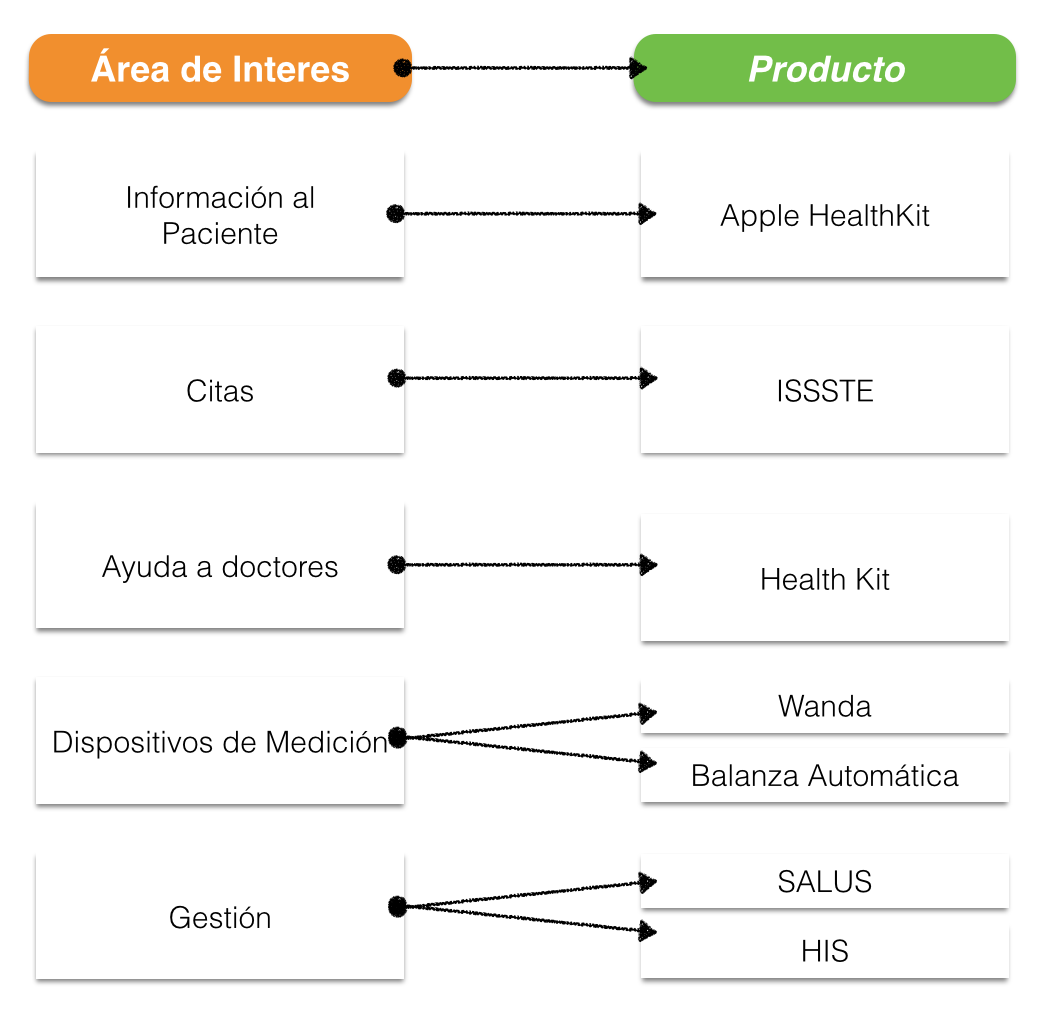
\includegraphics[height=11cm]{res-benchmarking.png}
\caption{Descripci�n gr�fica de las �reas de inter�s en la investigaci�n de \emph{benchmarking}.}
\label{fig:res-benchmarking}
\end{center}
\end{figure}

Seguido se procedi� con la realizaci�n de las entrevistas semi-estructuradas (Cuadro \ref{tab:resultados-num_entrevistador}), dando un total de siete personas. Cada una de las entrevistas tuvo una duraci�n de aproximadamente treinta minutos. Por otro lado, los resultados cualitativos de las entrevistas realizadas se pueden observar en la secci�n de Anexos (codificaci�n de entrevistas semi-estructuradas). 

\begin{table}[h]
	\caption{N�mero de personas y codificaciones por perfil entrevistado.}
	\label{tab:resultados-num_entrevistador}
	\centering
	\begin{tabular}{p{5cm} c c}
		\hline
		\multirow{2}{4.5cm}{Perfil} & Cantidad de personas  & Cantidad de codificaciones\\
		& $n=7$ & $n=112$\\
		\hline
		\hline
		M�dico & 3 (43\%) & 70 (62\%) \\
		Enfermera/o & 2 (29\%) & 28 (25\%) \\
		Encargado del paciente & 1 (14\%) & 02 (02\%) \\
		Administrativo (Archivo, Farmacia e inform�tica) & 1 (14\%) & 12 (11\%) \\
		\hline
	\end{tabular}
\end{table}

A partir del Cuadro \ref{tab:resultados-num_entrevistador}, es posible observar que diferentes perfiles aportaron una cantidad distinta de codificaciones. Para una visualizaci�n m�s explicita se presentan los resultados mediante el siguiente gr�fico de pie (Figura \ref{fig:codificaciones}); el mismo ofrece una panor�mica visual y detallado de las codificaciones obtenidas a partir de los perfiles evaluados.\\

\begin{figure}[h]
	\begin{center}
		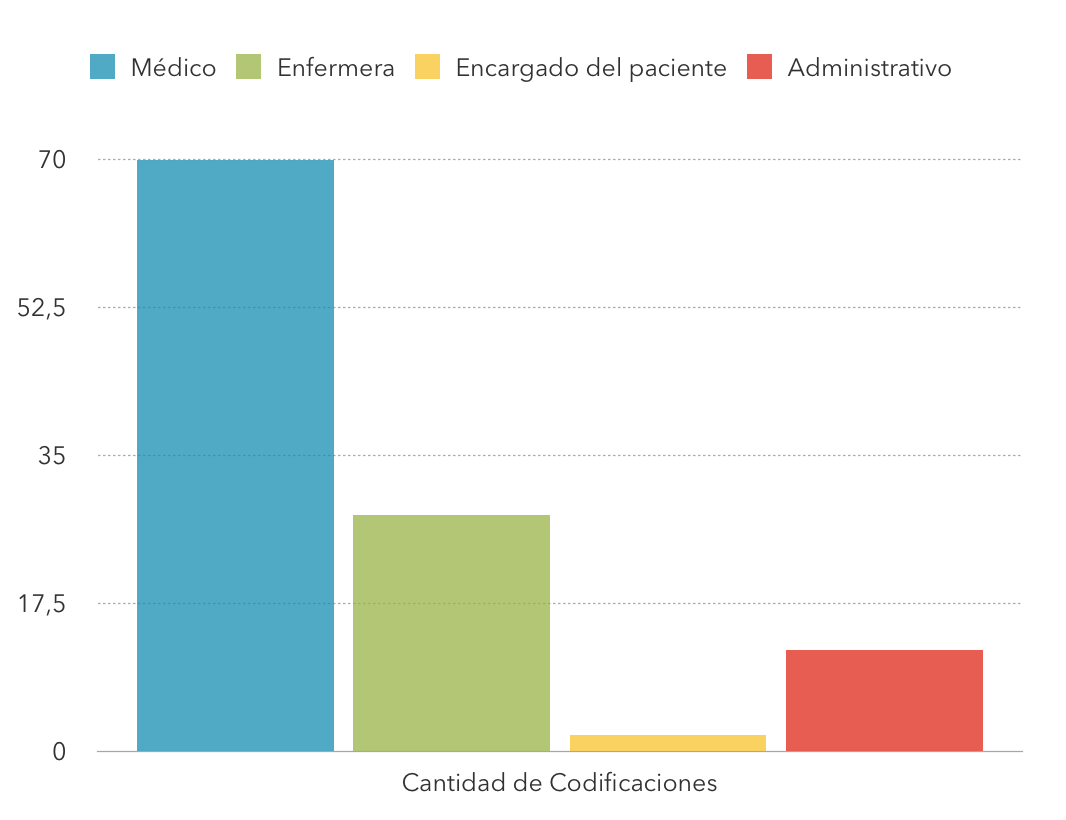
\includegraphics[height=6cm]{codificaciones.png}
		\caption{Cantidad de codificaciones por perfil.}
		\label{fig:codificaciones}
	\end{center}
\end{figure}

El contenido de las entrevistas por ser de tipo semi-estructuradas, no pueden ser resumidas en una sola tabla, ya que las preguntas eran abiertas y daban lugar a que los perfiles relataran historias o hechos. Sin embargo, se pueden resaltar algunas para que el lector tenga una idea sobre las ideas mencionadas:\\

\Citar{Pre-clasificaci�n pasa a admisi�n [...] pero es un paso muerto [porque se tienen igual que dar el n�mero de la cl�nica]. [...] Adem�s nosotros nos volvemos preclasificadores [cuando el paciente se env�a a una cl�nica err�nea].}
\Citar{Todo [el registro de datos del paciente] lo hacemos a mano.}
\Citar{Cada visita que viene el paciente se le pesa y se le talla. A menos que tenga menos de un mes de haber venido.}
\Citar{Si me toca perder la cita, tengo que volver a sacar una nueva en el hospital.}

%S�ntesis
\section{S�ntesis}

Despu�s de la separaci�n iterativa de los temas, se lleg� a la determinaci�n de un total de 11 temas generales en el hospital. El Cuadro \ref{tab:resultados-sintesis-grupos} muestra la proporci�n de codificaciones, por perfil, pertenecientes a cada tema. Este permite observar m�s a detalle la relevancia de cada uno de los mismos con los usuarios objetivo.

\begin{table}[ht]
	\caption{Proporci�n de codificaciones por perfil en temas generales.}
	\label{tab:resultados-sintesis-grupos}
	\centering
	\begin{tabular}{l | c c c c}
		\hline
		\multirow{3}{*}{Tema} & \multicolumn{4}{c}{Codificaciones por perf�l} \\
		\cline{2-5}
		& M�dico & Enfermera/o & Paciente & Administrativo \\
		& $n = 70$ & $n=28$ & $n=2$ & $n=12$\\
		\hline
		\hline
		Documentos de Procesos	& 08 (12\%) & 3 (11\%) & 0 (00\%) & 0 (00\%)\\
		Datos del Paciente 		& 09 (13\%) & 0 (00\%) & 0 (00\%) & 3 (25\%)\\
		Comunicaci�n 			& 05 (07\%) & 1 (04\%) & 0 (00\%) & 0 (00\%)\\
		Documentos a Mano	 	& 05 (07\%) & 4 (14\%) & 0 (00\%) & 0 (00\%)\\
		Citas 					& 03 (04\%) & 1 (04\%) & 1 (50\%) & 0 (00\%)\\
		Expediente 				& 06 (09\%) & 3 (11\%) & 0 (00\%) & 2 (17\%)\\
		Tecnolog�a 				& 05 (07\%) & 7 (24\%) & 0 (00\%) & 0 (00\%)\\
		Necesidad del personal 	& 05 (07\%) & 3 (11\%) & 0 (00\%) & 1 (08\%)\\
		Necesidad de los pacientes & 06 (09\%) & 1 (04\%) & 1 (50\%) & 2 (17\%)\\
		Procesos 				& 11 (15\%) & 4 (14\%) & 0 (00\%) & 4 (33\%)\\
		Referencias 			& 06 (09\%) & 0 (00\%)& 0 (00\%) & 0 (00\%) \\
		Sin Tema & 01 (01\%) & 1 (04\%) & 0 (00\%) & 0 (00\%)\\
		\hline
	\end{tabular}
\end{table}

A partir de la separaci�n de temas, a cada uno fue posible determinar un conjunto de \emph{insigth}. Adem�s como �ltimo paso, tambi�n se determinaron las oportunidades de dise�o de cada uno. El Cuadro \ref{tab:res-sintesis-num} muestra los resultados de una forma cuantitativa.\\


\begin{table}[ht]
	\caption{Proporci�n de \emph{insights} y codificaciones encontradas por cada tema.}
	\label{tab:res-sintesis-num}
	\centering
	\begin{tabular}{l | c c}
		\hline
		\multirow{2}{*}{Tema} & \emph{Insights} & Oportunidades \\
		& $n = 26$ & $n=13$\\
		\hline
		\hline
		Documentos a Mano & 2 (08\%) & 1 (08\%)\\
		Datos del Paciente 		& 3 (11\%) & 1 (08\%)\\
		Comunicaci�n 			& 3 (11\%) & 1 (08\%)\\
		Documentos de Procesos 	& 2 (08\%) & 1 (08\%) \\
		Citas 					& 3 (11\%) & 1 (08\%)\\
		Expediente 				& 4 (16\%) & 3 (22\%)\\
		Tecnolog�a 				& 3 (11\%) & 2 (14\%)\\
		Necesidad del personal 	& 1 (04\%) & 1 (08\%)\\
		Necesidad de los pacientes & 2 (08\%) & 1 (08\%)\\
		Procesos 				& 2 (08\%) & 1 (08\%)\\
		Referencias 			& 1 (04\%) & 0 (00\%)\\

		\hline
	\end{tabular}
\end{table}

Por otra parte, la Figura \ref{fig:res-sintesis} muestra tales resultados de una forma gr�fica, con una breve descripci�n de cada uno de los productos generados.\\

\begin{figure}[ht]
	\begin{center}
		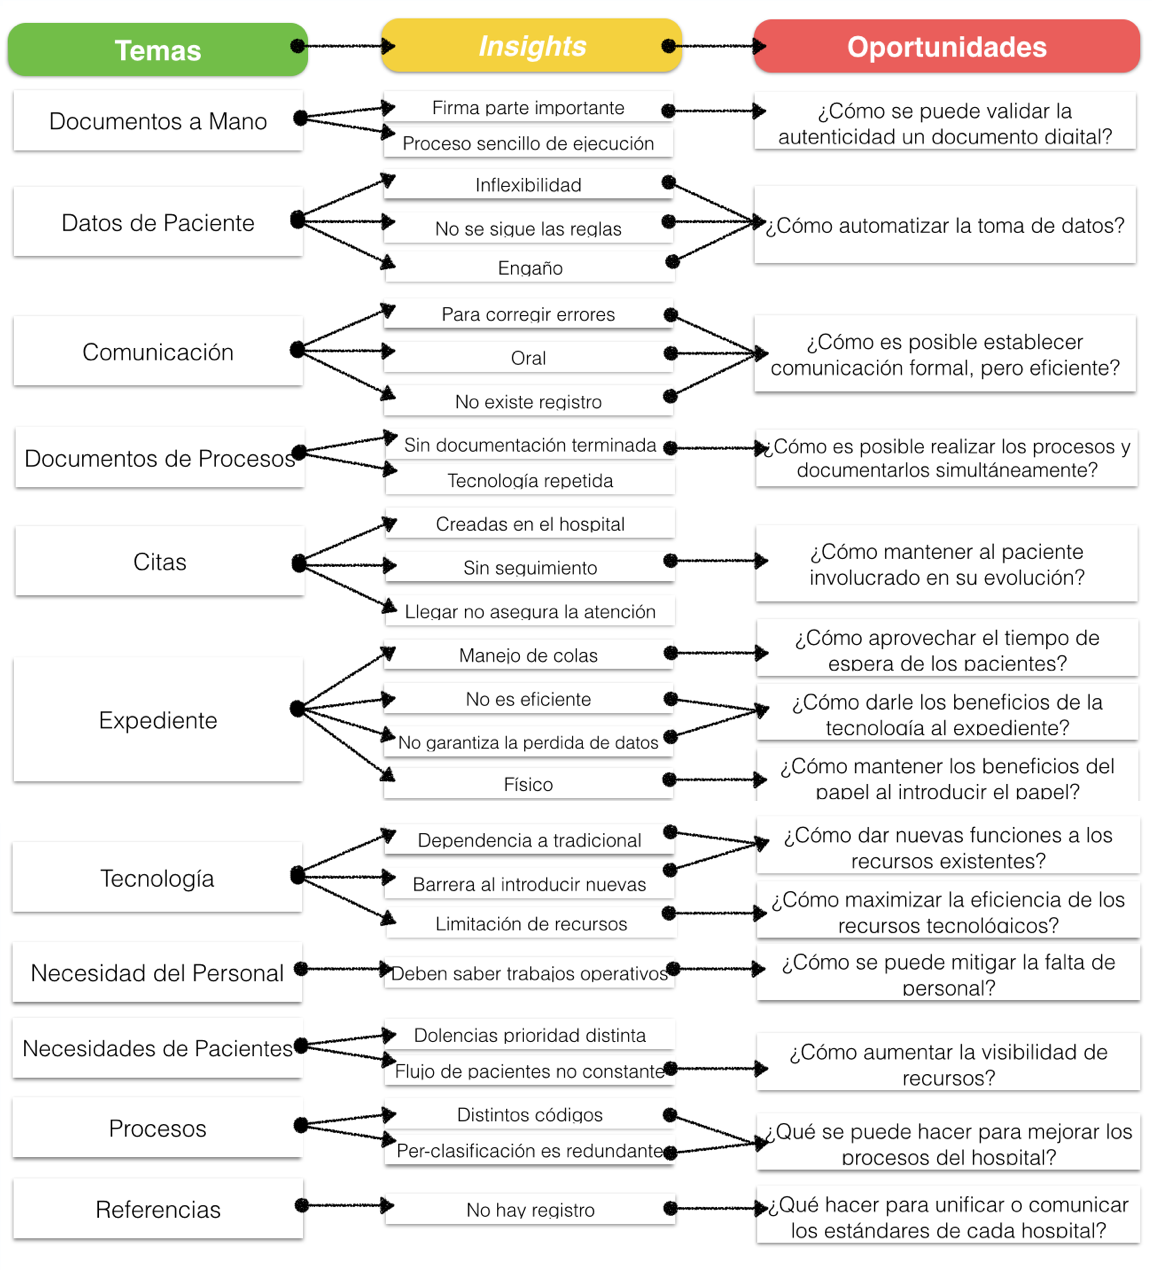
\includegraphics[width=15cm]{res-sintesis.png}
		\caption{Evoluci�n de temas a \emph{insights} y a oportunidades de dise�o.}
		\label{fig:res-sintesis}
	\end{center}
\end{figure}

%Exploraci�n
\section{Exploraci�n}
A partir de las oportunidades de dise�o de la etapa anterior, se dise�aron una serie de propuestas soluci�n en un lluvia de ideas. El contenido completo de todas las propuestas se muestra en la secci�n de Anexos (lluvia de ideas) y el Cuadro \ref{tab:resultados-expl} muestra un resumen.\\

\begin{table}[ht]
\caption{Cantidad de propuestas por oportunidad}
\label{tab:resultados-expl}
\centering
\begin{tabular}{p{10cm} c}
\hline
\multirow{2}{*}{Oportunidad} & Ideas de dise�o \\
 & $n=174$ \\
 \hline\hline
�C�mo se puede validar la autenticidad de un documento digital? & 15 (9\%)\\
�C�mo automatizar la toma de datos? & 14 (8\%) \\
�C�mo es posible establecer comunicaci�n formal, pero eficiente? & 10 (6\%)\\
�C�mo es posible realizar los procesos y documentarlos de manera simult�nea? & 13 (7\%)\\
�C�mo mantener al paciente involucrado en su evoluci�n? & 16 (9\%) \\
�C�mo aprovechar el tiempo de espera de los pacientes? & 14 (8\%)\\
�C�mo darle los beneficios que ofrece la tecnolog�a al expediente? & 13 (7\%)\\
�C�mo mantener los beneficios del papel al introducir tecnolog�a? & 09 (5\%)\\
�C�mo dar nuevas funciones a los recursos existentes? & 12 (7\%)\\
�C�mo maximizar la eficacia de los recursos tecnol�gicos? & 11 (6\%)\\
�C�mo se puede mitigar la falta de personal usando tecnolog�a? & 13 (7\%)\\
�C�mo aumentar la visibilidad para la gesti�n de recursos? & 14 (8\%)\\
�C�mo mantener el expediente actualizado a lo largo del proceso? & 14 (8\%)\\
�Qu� hacer para unificar o comunicar los est�ndares de cada hospital? & 06 (5\%)\\
\hline
\end{tabular}
\end{table}
Para brindarle al lector una mejor visualizaci�n de la forma en que se generaron las ideas de dise�o, a continuaci�n se muestran algunas ideas que fueron seleccionadas para un posible prototipo (Figura \ref{fig:res-exploracion}).\\

\begin{figure}[ht]
	\begin{center}
		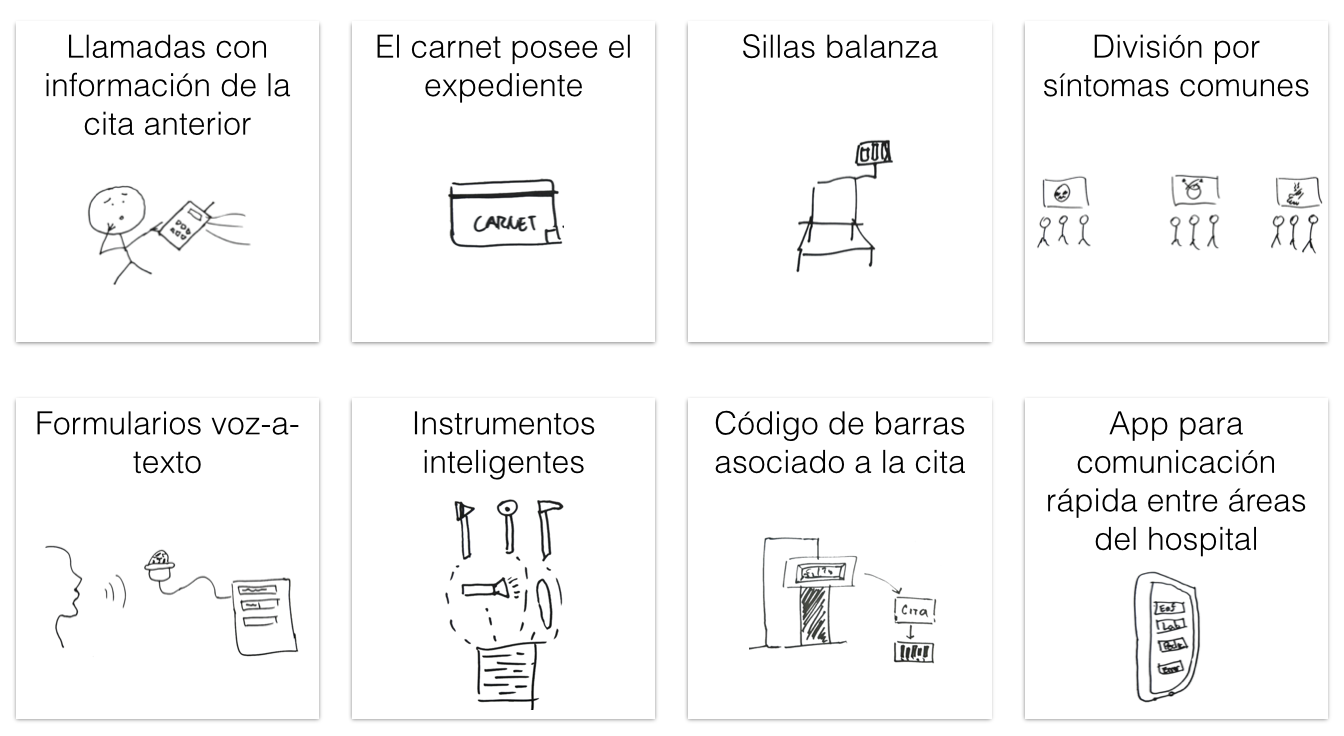
\includegraphics[height=7cm]{res-exploracion.png}
		\caption{Ejemplos de ideas de dise�o generadas en la lluvia de ideas.}
		\label{fig:res-exploracion}
	\end{center}
\end{figure}

%Dise�o de Prototipos
\section{Dise�o de Prototipos}

La primera fase del dise�o de prototipos llev� a una votaci�n de todas las ideas generadas en el proceso anterior. A partir de tales votaciones, se eligieron cinco ideas de dise�o, las cuales se convirtieron en los m�dulos a trabajar por cada uno de los integrantes del grupo (Figura \ref{fig:modulos}).

\begin{figure}[ht]
	\begin{center}
		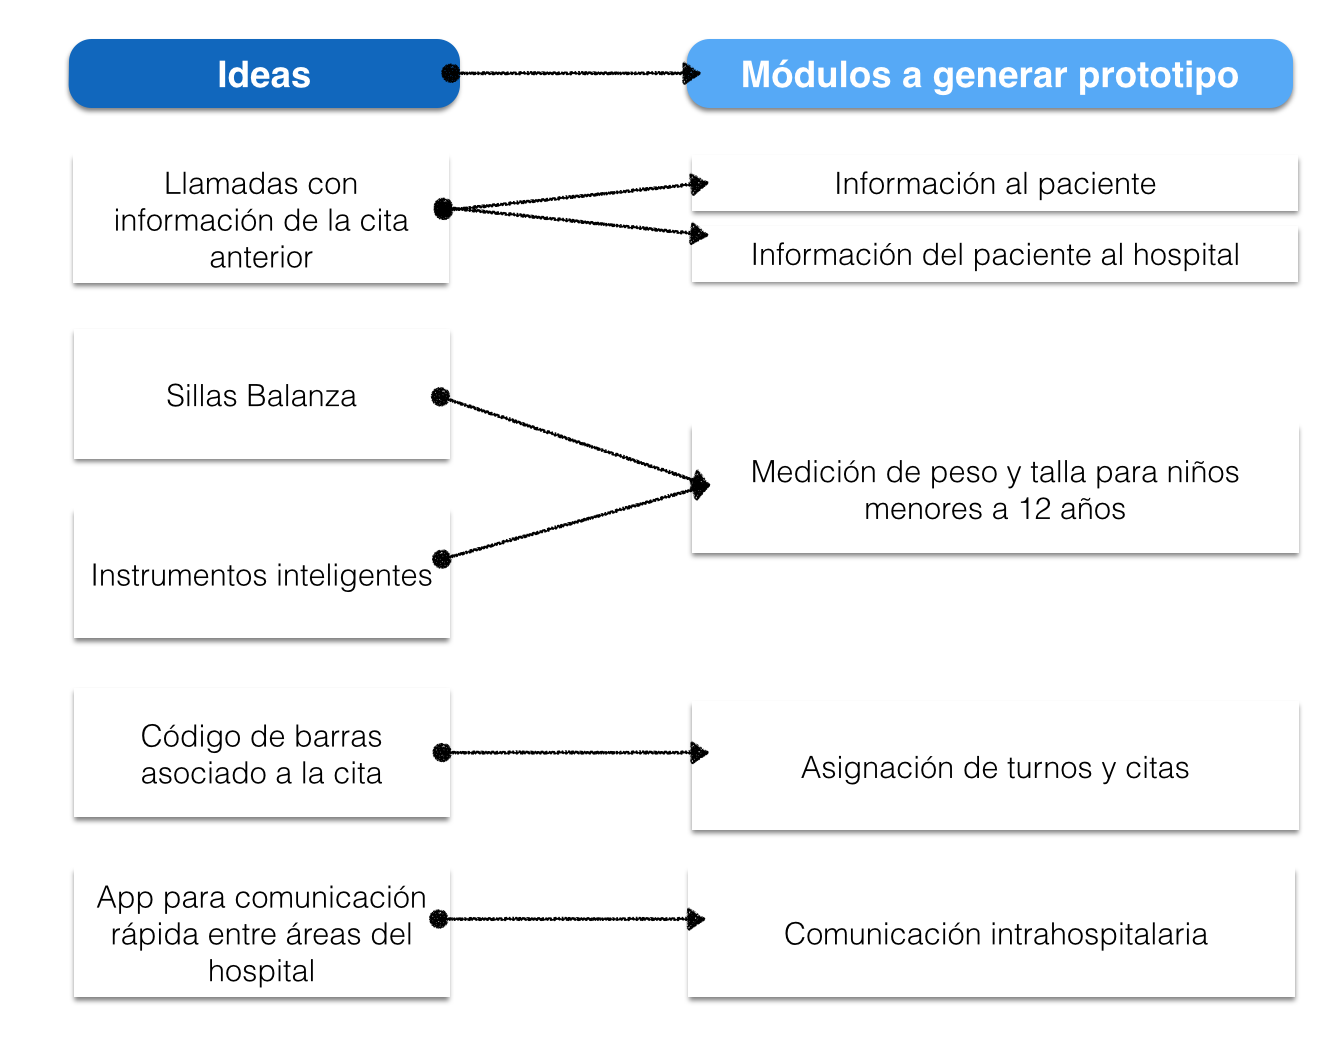
\includegraphics[height=8cm]{modulos.png}
		\caption{Ideas de dise�o tomadas en cuenta para la generaci�n de m�dulos trabajadas.}
		\label{fig:modulos}
	\end{center}
\end{figure}

Con la generaci�n de la idea de los m�dulos, cada integrante comenz� con el trabajo de los prototipos. Debido a problemas con el ingreso a los hospitales p�blicos, el estudio se extendi� a tres hospitales. Para la demostraci�n de las �reas que se encontraron en com�n, a partir de entrevistas realizadas en los hospitales de: Infectolog�a y Rehabilitaci�n, San Juan de Dios y Roosevelt; se realiz� una matriz de calor descrita en la Figura \ref{fig:hospitales}. Para una observaci�n completa de tales entrevistas, es posible referirse a la secci�n de anexos (entrevistas comparativas de hospitales).

\begin{figure}[ht]
	\begin{center}
		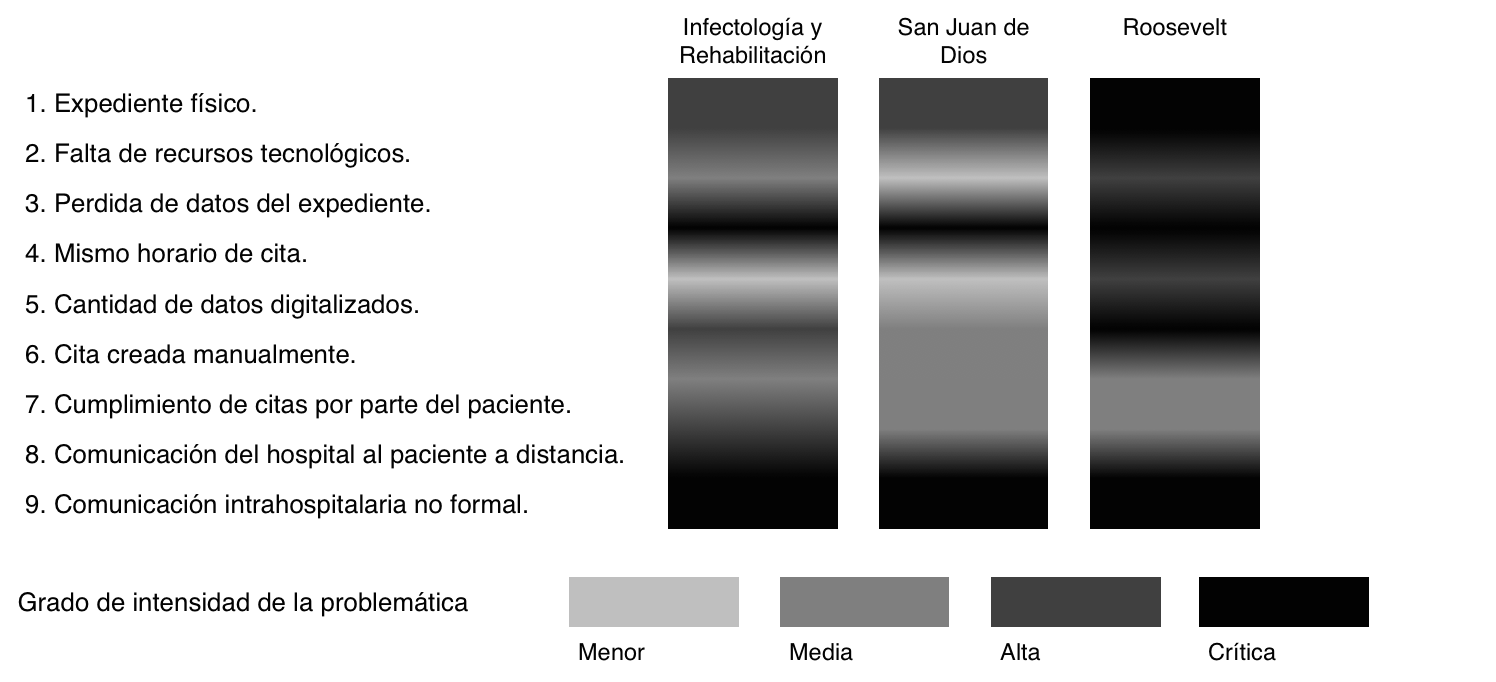
\includegraphics[width=10.3cm]{comparacion-hospitales.png}
		\caption{Matriz de calor de �reas en com�n para los hospitales trabajados.}
		\label{fig:hospitales}
	\end{center}
\end{figure}

Cada integrante se comenz� a especializar en el m�dulo que escogi�, por lo tanto de las 5 ideas generadas, este trabajo realiz� sus validaciones �nicamente en base al m�dulo de informaci�n al paciente. En la siguiente secci�n se detallan los resultados de el proceso de refinado de los prototipos con cada uno de los perfiles. Adem�s, se presenta la forma en que el prototipo refinado resultante se puede realizar.\\ 


%Andrea
\subsection{Validaci�n externa del m�dulo informaci�n al paciente}

En esta secci�n se comienza con una de las fases m�s importantes para el dise�o del sistema de informaci�n al paciente, ya que gracias a los resultados de estas validaciones se tomaron decisiones claves. Para la validaci�n interna de los prototipos, los cambios solicitados fueron m�nimos: cambios en redacci�n, presentaci�n de los dibujos y nombres de los integrantes de la historia de usuario. Por ello, no se realiz� un cap�tulo que hablara solamente de ellos. Sino que a continuaci�n se presentan los resultados importantes encontrados en las validaciones externas.\\ 


\subsubsection{Validaci�n de los \emph{storyboards}}

 El Cuadro \ref{tab:sms-externo}, muestra los resultados de las iteraciones externas en las cuales se valid� el prototipo de baja fidelidad del env�o de SMS. Con el fin de no mostrar las 3 versiones del \emph{storyboard}, se identificaron los temas que m�s recib�an retroalimentaci�n. Para esto, se estableci� un \checkmark si el tema se encontraba correctamente representado y una $x$ si no. Para m�s detalles de la raz�n por la que se colocaron estos valores, revisar el an�lisis de resultados. \\
 
 
\begin{table}[ht]
	\caption{Iteraciones externas del \emph{storyboard} de baja fidelidad del tema SMS}
	\label{tab:sms-externo}
	\centering
	\begin{tabular}{l | c c c}
		\hline
		Tema & Iteraci�n 1 & Iteraci�n 2 & Iteraci�n 3 \\
		\hline
		\hline
		Llegada del paciente al hospital & \checkmark & $x$ & \checkmark\\
		Indicaciones del doctor & \checkmark & $x$ & \checkmark\\
		Env�o del SMS de medicina & \checkmark & $x$ & $x$\\
		Paciente adquiere medicina & \checkmark & \checkmark & $x$\\
		Env�o del SMS de documentos & \checkmark & $x$ & $x$\\
		Env�o del SMS de citas & \checkmark & \checkmark & $x$\\
		Retroalimentaci�n para el hospital & \checkmark & \checkmark & \checkmark\\
		\hline
	\end{tabular}
\end{table}


De la misma forma se realizaron las validaciones del \emph{storyboard} que conten�a la historia que involucra el uso del IVR ver Cuadro \ref{tab:ivr-externo}. Estas iteraciones se realizaron con las mismas personas que en la anterior. En esta historia no se incluyen los temas en relaci�n a la llegada del paciente al hospital, ya que estos fueron considerados en el \ref{tab:sms-externo} anterior. \\ \\ \\


\begin{table}[ht]
	\caption{Iteraciones externas del \emph{storyboard} de baja fidelidad del tema IVR}
	\label{tab:ivr-externo}
	\centering
	\begin{tabular}{l | c c c}
		\hline
		Tema & Iteraci�n 1 & Iteraci�n 2 & Iteraci�n 3 \\
		\hline
		\hline
		Contenido de la llamada de medicina & \checkmark & $x$ & \checkmark\\
		Contenido de la llamada de documentos & \checkmark & $x$ & \checkmark\\
		Contenido de la llamada de citas & \checkmark & \checkmark & \checkmark\\
		Interacci�n paciente con IVR & \checkmark & $x$ & $x$\\
		\hline
	\end{tabular}
\end{table}


Para finalizar la primera etapa de validaci�n de prototipos de baja fidelidad, se procedi� a mostrar el \emph{storyboard} el cual utiliza una aplicaci�n m�vil como medio de comunicaci�n. Para ello ver el Cuadro \ref{tab:app-externo} el cual muestra los resultados de los temas m�s comentados por parte de los usuarios.
\begin{table}[ht]
	\caption{Iteraciones externas del \emph{storyboard} de baja fidelidad del tema aplicaci�n m�vil}
	\label{tab:app-externo}
	\centering
	\begin{tabular}{l | c c c}
		\hline
		Tema & Iteraci�n 1 & Iteraci�n 2 & Iteraci�n 3 \\
		\hline
		\hline
		Comprensi�n del concepto de aplicaci�n & $x$ & $x$ & \checkmark\\
		Comprensi�n del men� principal & \checkmark & \checkmark & \checkmark\\
		Interacci�n con pesta�a de citas & \checkmark & \checkmark & \checkmark\\
		\hline
	\end{tabular}
\end{table}

A cada una de las personas entrevistadas durante las iteraciones, se les pregunt� cu�l de los tres \emph{storyboards} preferir�an. El Cuadro \ref{tab:votacion-externo} muestra los resulados de las preferencias y las combinaciones que crearon. Para la soluci�n que incluye aplicaci�n m�vil y SMS, especificaron que la aplicaci�n la prefer�an para confirmar la llegada a la cita. En el caso de IVR con aplicaci�n m�vil, utilizar las llamadas para confirmarla. Por �ltimo, 2 indicaron nuevamente que prefer�an la llamada para el recordatorio de cita.\\
\begin{table}[ht]
	\caption{Resultado de votaciones por tema de \emph{storyboard}}
	\label{tab:votacion-externo}
	\centering
	\begin{tabular}{l | c c}
		\hline
		Tema por \emph{storyboard} & No. Votos & Justificaci�n en com�n de la decisi�n\\
		\hline
		\hline
		 SMS & 3 & El contenido queda guardado como respaldo. \\
		 IVR & 1 & Recuerdo el contenido f�cilmente. \\
		 aplicaci�n m�vil & 0 & Escasos recursos. \\
		 aplicaci�n m�vil y SMS & 1 & No se gasta en saldo para confirmar la cita. \\
		 aplicaci�n m�vil e IVR & 1 & Para poder explicar la raz�n por la que no voy a ir.\\
		 IVR y SMS & 2 & Para confirmar la cita con la llamada.  \\
		\hline
	\end{tabular}
\end{table}

 \subsubsection{Entrevistas a pacientes}

Como resultado de las tres iteraciones que se realizaron m�s los datos recopilados en las iteraciones, se lleg� a una versi�n final de cada \emph{storyboard}. Luego, en base a estas versiones finales, se redact� una entrevista semi-estructurada con el fin de evaluar el medio de comunicaci�n m�s adecuado para el paciente.\\

Los dos m�dulos de informaci�n entre el paciente y el hospital realizaron la entrevista adicional para conseguir informaci�n que permitiera determinar el acercamiento a cada m�dulo. El formato de las entrevistas puede verse en la secci�n de Anexos (entrevistas sobre comunicaci�n de pacientes). Los resultados obtenidos se pueden ver en las siguientes tablas.\\ 
 
 La entrevista cont� con una serie de preguntas generales Cuadro \ref{tab:entrev-comm-pg}, en las se pretend�a identificar a qu� tipo de tecnolog�a tienen acceso los pacientes en todo momento. Identificar si primero ten�an un celular, y si era afirmativo, qu� tipo y con qu� capacidades. En base a estos resultados, se conmenzaron las otras secciones de preguntas de la entrevista.\\ 
 
 
 \begin{table}[h]
 	\caption{Preguntas Generales}
 	\label{tab:entrev-comm-pg}
 	\centering
 	\begin{tabular}{p{6cm} p{2cm} p{3cm} p{2cm} }
 		\hline
 		Pregunta & Muestra & Respuestas & Porcentaje \\
 		\hline\hline
 		\multirow{3}{6cm}{1. �Qu� tel�fono m�vil posee?} & 	\multirow{3}{2cm}{n=25} & Inteligente & 44\% \\
 		&						&	No inteligente & 52\% \\
 		&						&	Ninguno & 4\% \\ \hline
 		\multirow{4}{6cm}{3. �Qu� medio usa m�s para comunicarse con profesionales?} & \multirow{4}{2cm}{n=25} & Llamada & 36\% \\
 		&						&	Habla en persona & 12\% \\
 		&						&	Web	& 4\% \\
 		&						&	Ninguno & 48\% \\ \hline
 		\multirow{4}{6cm}{4. �Qu� medio usa m�s para comunicarse con amigos/familia?} & \multirow{4}{2cm}{n=25} & Llamada & 80\% \\
 		&						&	Habla en persona & 4\% \\
 		&						&	Redes sociales	& 12\% \\
 		&						&	Chat & 8\% \\ \hline
 		\multirow{5}{6cm}{5. �Responde siempre las llamadas que recibe?} & \multirow{5}{2cm}{n=25} & S� & 52\% \\
 		&						&	No & 8\% \\
 		&						&	A veces	& 28\% \\
 		&						&	Depende & 8\% \\
 		&						&	No recibo & 4\% \\ \hline
 		\multirow{5}{6cm}{6. �Qu� medio usa para responder llamadas?} & \multirow{5}{2cm}{n=25} & Llamada & 64\% \\
 		&						&	SMS & 8\% \\
 		&						&	Espera otra	& 8\% \\
 		&						&	NS/NR & 4\% \\
 		&						&	Ninguno & 16\% \\ \hline
 		\multirow{5}{6cm}{7. �Qu� medio usa para responder SMS?} & \multirow{5}{2cm}{n=25} & Llamada & 32\% \\
 		&						&	SMS & 40\% \\
 		&						&	Otros	& 4\% \\
 		&						&	NS/NR & 12\% \\
 		&						&	Ninguno & 12\% \\ \hline
 		\multirow{5}{6cm}{8. �Qu� tan seguido se conecta a internet?} & \multirow{5}{2cm}{n=13} & 30 d�as/mes & 46.7\% \\
 		&						&	16 d�as/mes & 6.7\% \\
 		&						&	12 d�as/mes	& 6.7\% \\
 		&						&	2 d�as/mes & 20\% \\
 		&						&	1 d�a/mes & 20\% \\ \hline
 		\multirow{3}{6cm}{10. �Para qu� usa m�s su tel�fono, Llamadas o SMS?} & \multirow{3}{2cm}{n=13} & Llamadas & 72\% \\
 		&						&	SMS & 12\% \\
 		&						&	Ninguno	& 16\% \\ 
 		\hline \\ \\ \\ \\
 	\end{tabular}
 \end{table}
 
 
 La pregunta 2 del tema ``Preguntas Generales'' es ilustrada por la gr�fica jer�rquica en \ref{fig:entrevistas-pg2}. Muestra todas las diversas respuestas que se obtuvieron de la pregunta 2. Para entender mejor todas las posibilidades, se decidi� representarlo de esta manera para que sea m�s comprensible para el lector. El grupo de llamar (8\%) queda exclu�do por completo de los grupos principales que son Internet e ir a preguntar.\\ 
 
 \begin{figure}[h]
 	\begin{center}
 		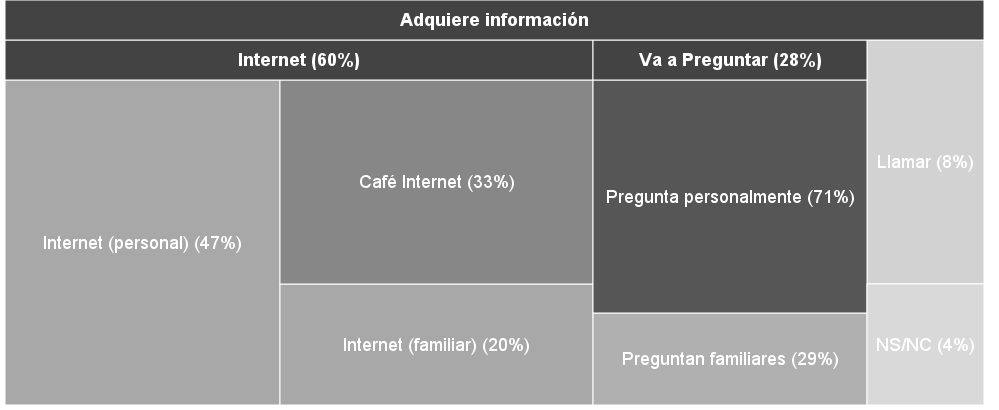
\includegraphics[height=6.2cm]{res-entrev-pg2.png}
 		\caption{Preguntas Generales 2. ``�Qu� hace cuando necesita informaci�n?''}
 		\label{fig:entrevistas-pg2}
 	\end{center}
 \end{figure}
 
 Los Cuadros \ref{tab:entrev-comm-ns} y \ref{tab:entrev-comm-ss}, muestran los resultados de las preguntas relacionadas al tipo de m�vil que poseen los pacientes. El objetivo de estas preguntas era identificar que independientemente del celular que tengan, verificar qu� otros medios podr�an estar utilizando para comunicarse.\\  
 
 
 \begin{table}[h]
 	\caption{Preguntas para tel�fonos no inteligentes}
 	\label{tab:entrev-comm-ns}
 	\centering
 	\begin{tabular}{p{6cm} p{2cm} p{3cm} p{2cm} }
 		\hline\hline
 		Pregunta & Muestra & Respuestas & Porcentaje \\
 		\hline
 		\multirow{3}{6cm}{1. �Tiene otro medio de comunicaci�n?} & 	\multirow{3}{2cm}{n=25} & S� & 0\% \\
 		&						&	No & 52\% \\
 		&						&	No aplica & 48\% \\ 
 		\hline \\ \\ \\ \\ \\ \\ \\ \\ \\ \\ \\ \\ \\
 		
 	\end{tabular}
 \end{table}
 
 \begin{table}[h]
 	\caption{Preguntas para tel�fonos inteligentes}
 	\label{tab:entrev-comm-ss}
 	\centering
 	\begin{tabular}{p{6cm} p{1.5cm} p{3.5cm} p{2cm} }
 		\hline
 		Pregunta & Muestra & Respuestas & Porcentaje \\
 		\hline\hline
 		\multirow{3}{6cm}{1. �Si le van a dar informaci�n prefiere llamadas, SMS o una aplicaci�n con alarmas?} & 	\multirow{3}{2cm}{n=18} & Llamada & 44.4\% \\
 		&						&	SMS & 44.4\% \\
 		&						&	Alarmas & 11.2\% \\ \hline
 		\multirow{6}{6cm}{2. �Qu� aplicaciones para comunicarse usan?} & 	\multirow{6}{2cm}{n=11} & WhatsApp & 36.4\% \\
 		&						&	Facebook & 9.05\% \\
 		&						&	Ninguna & 27.3\% \\
 		&						&	WhatsApp, FB & 18.2\% \\
 		&						&	WhatsApp, MSN, Line & 9.05\% \\ \hline
 		\hline
 	\end{tabular}
 \end{table}
 
Para verificar si era viable enviarles recordatorios por medio de correo electr�nico, se les realiz� las siguientes preguntas (Cuadro \ref{tab:entrev-comm-ai}). No se incluyen los resultados de la pregunta 2 y 4, ya que no se consideran relevantes para la l�nea de comunicaci�n que surge del hospital hacia el paciente.\\ 
 
 \begin{table}[h]
 	\caption{Preguntas sobre acceso a Internet}
 	\label{tab:entrev-comm-ai}
 	\centering
 	\begin{tabular}{p{6cm} p{2cm} p{3cm} p{2cm} }
 		\hline
 		Pregunta & Muestra & Respuestas & Porcentaje \\
 		\hline\hline
 		\multirow{7}{6cm}{1. �Qu� tan seguido suele recibir informaci�n por correo electr�nico?} & 	\multirow{7}{2cm}{n=21} & No tiene e-mail & 52.4\% \\
 		&						&	No recibe & 19\% \\
 		&						&	Cada 3 semanas & 4.8\% \\
 		&						&	Todos los d�as & 9.4\% \\
 		&						&	Casi nunca & 4.8\% \\
 		&						&	Cada 2 semanas & 4.8\% \\
 		&						&	Poco & 4.8\% \\ \hline
 		\multirow{4}{6cm}{4. �Tiene redes sociales? Si s�, �cu�les?} & 	\multirow{4}{2cm}{n=25} & No tiene & 59.09\% \\
 		&						&	Facebook & 31.82\% \\
 		&						&	FB y Twitter & 4.55\% \\
 		&						&	FB y Line & 4.54\% \\
 		\hline\hline
 	\end{tabular}
 \end{table}
 
 
 Por �ltimo, se realiz� una secci�n de preguntas para identificar de qu� forma usualmente los pacientes recuerdan la informaci�n importante que se les brinda en el hospital (Cuadro \ref{tab:entrev-comm-ri}).\\ \\ \\ \\ \\ \\ \\ \\ \\ \\ \\  
 
 \begin{table}[h]
 	\caption{Preguntas sobre recordatorios de informaci�n}
 	\label{tab:entrev-comm-ri}
 	\centering
 	\begin{tabular}{p{6cm} p{2cm} p{3cm} p{2cm} }
 		\hline
 		Pregunta & Muestra & Respuestas & Porcentaje \\
 		\hline\hline
 		\multirow{6}{6cm}{1. �Qu� hace para recordar una cita ya programada?} & 	\multirow{6}{2cm}{n=24} & Estar pendiente & 33.4\% \\
 		&						&	Alarma en el celular & 8.3\% \\
 		&						&	Apuntar en papel & 8.3\% \\
 		&						&	Carnet & 37.5\% \\
 		&						&	Se lo recuerdan & 4.2\% \\
 		&						&	Calendario & 8.3\% \\ \hline
 		\multirow{6}{6cm}{2. �Qu� hace para recordar los ex�menes que debe hacerse previo a una cita?} & \multirow{6}{2cm}{n=21} & Estar pendiente & 42.9\% \\
 		&						&	Alarma en el celular & 4.8\% \\
 		&						&	Apuntar en papel & 4.8\% \\
 		&						&	Carnet & 29\% \\
 		&						&	Se me olvida & 4.8\% \\
 		&						&	Calendario & 9.5\% \\ \hline
 		\multirow{5}{6cm}{3. �Qu� hace para recordar la medicina que debe tomar?} & \multirow{5}{2cm}{n=24} & Estar pendiente & 47.8\% \\
 		&						&	Alarma en el celular & 21.7\% \\
 		&						&	Apuntar en la caja & 8.7\% \\
 		&						&	Ver la medicina & 8.7\% \\
 		&						&	Ver la receta & 13\% \\ \hline
 		\hline
 	\end{tabular}
 \end{table}
 
 \begin{figure}[h]
 	\begin{center}
 		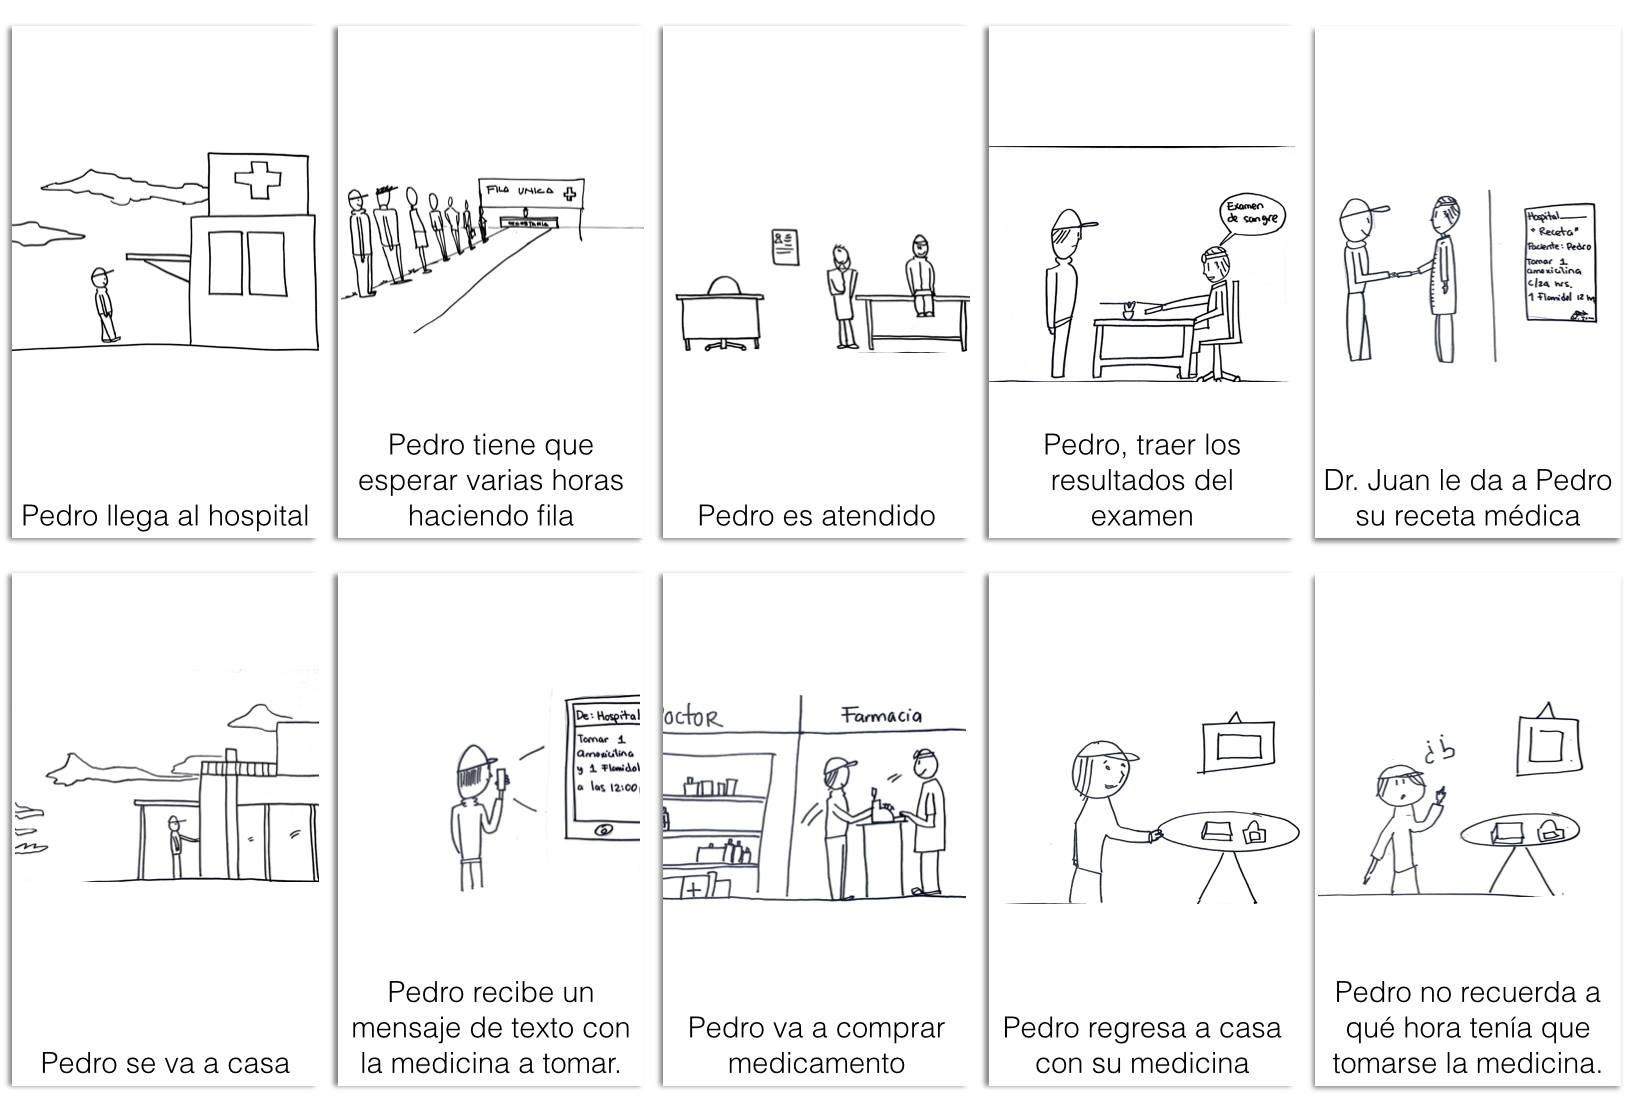
\includegraphics[height=5.6cm]{story1.jpg}
 		\caption{Versi�n final del prototipo de baja fidelidad del tema SMS}
 		\label{fig:baja-story}
 	\end{center}
 \end{figure}
 
  \begin{figure}[h]
  	\begin{center}
  		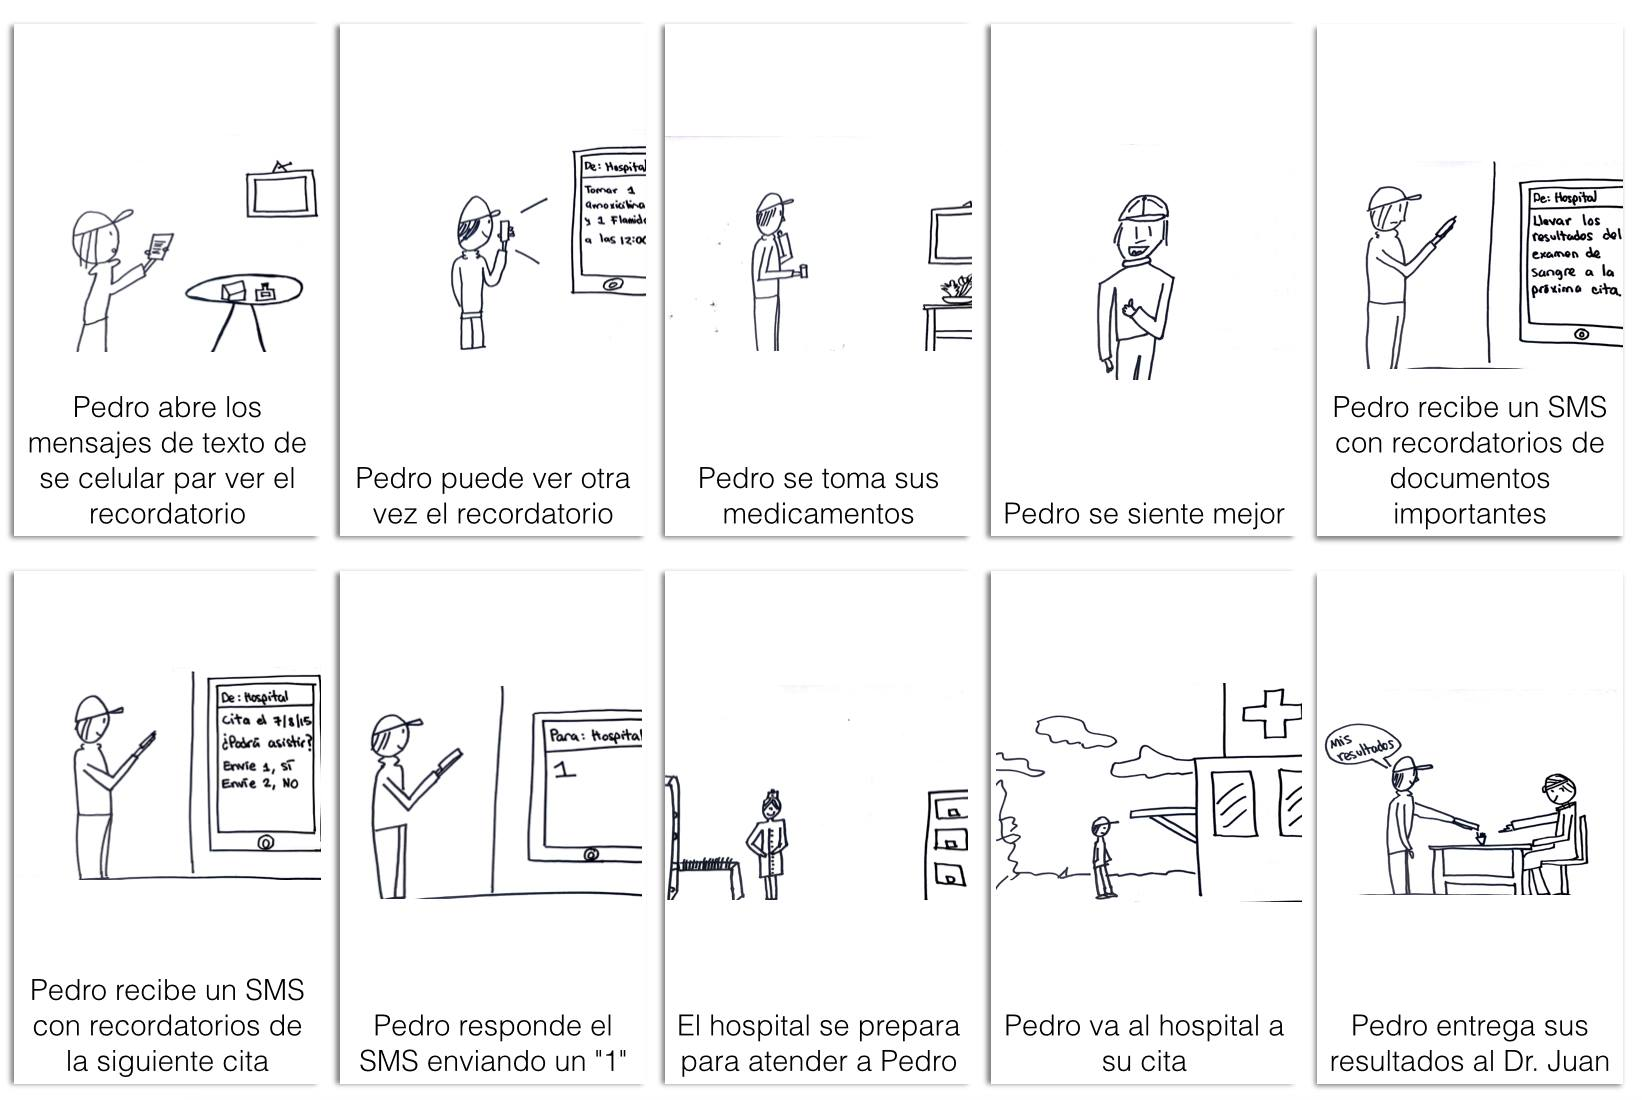
\includegraphics[height=5.6cm]{story2.jpg}
  		\caption{Continuaci�n de la Versi�n final del prototipo de baja fidelidad del tema SMS}
  		\label{fig:baja-story2}
  	\end{center}
  \end{figure}

Al analizar la informaci�n recopilada en las iteraciones y entrevistas, se escogi� el prototipo que utiliza el env�o de recordatorios por medio de SMS Figuras \ref{fig:baja-story} y \ref{fig:baja-story2}. A partir de esta versi�n final del prototipo de baja calidad, se procedi� a desarrollar los prototipos de mediana fidelidad.\\ \\ \\ \\ \\ \\ \\ \\ \\ 

\subsection{Investigaci�n de herramientas}

Para la fase de prototipos de mediana fidelidad, se realiz� una investigaci�n en la que se evaluaron varias plataformas de c�digo abierto que cumpl�an con los requisitos del \emph{storyboard} de env�o de SMS (Cuadro \ref{tab:open-mhealth}). Al final se eligi� la plataforma de c�digo abierto FrontlineSMS la cual cumple con todas las expectativas del prototipo de baja fidelidad.\\

Luego de haber elegido la plataforma de FrontlineSMS, se realizaron 2 visitas al Hospital Roosevelt para validar las pantallas de la aplicaci�n. Adicionalmente, se valid� el contenido de los recordatorios a enviar a los pacientes. Como resultado, se obtuvo el visto bueno del m�dico y la secretaria involucradas en el proceso de recordarle a los pacientes informaci�n. Las 2 pantallas principales de alta calidad del sistema de FrontlineSMS se pueden apreciar en las Figuras \ref{fig:frontline-sms1} y  \ref{fig:frontline-sms2}.\\

\begin{figure}[h]
      	\begin{center}
      		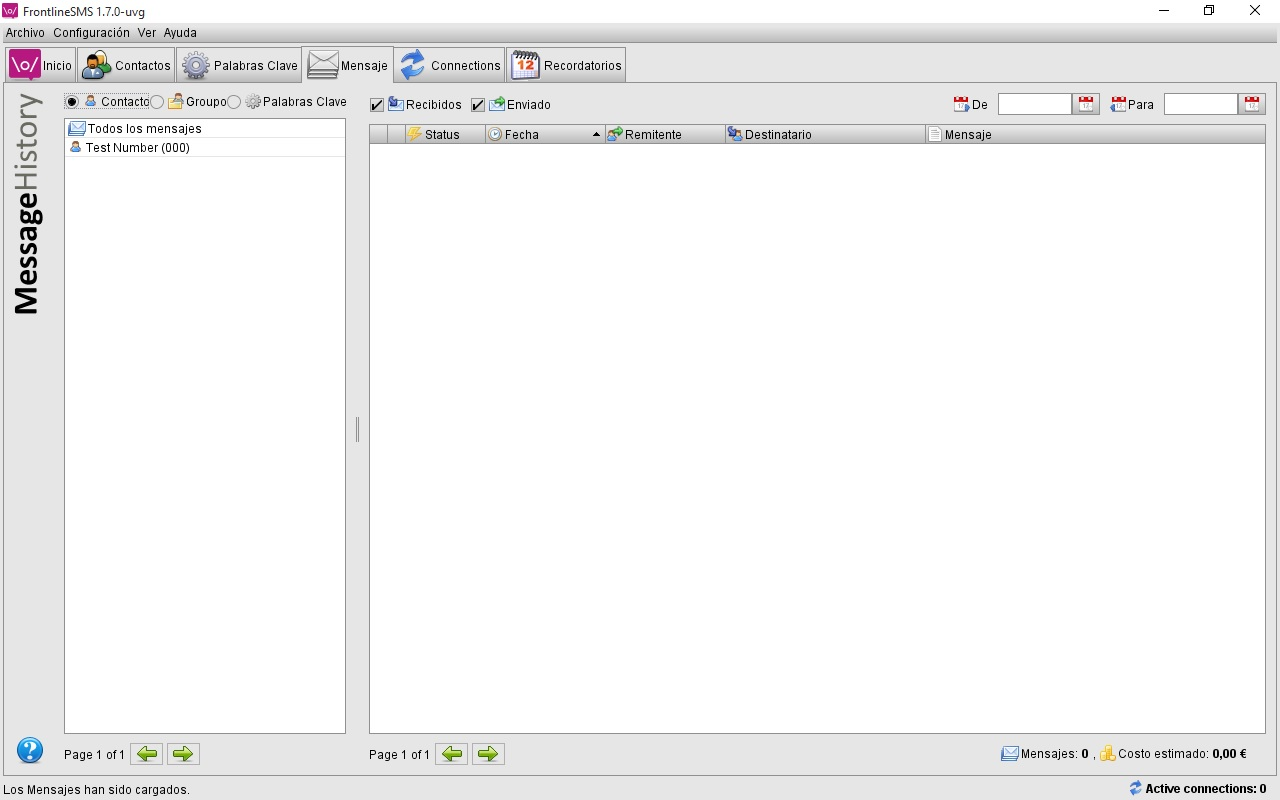
\includegraphics[height=7cm]{frontlinesms4.jpg}
      		\caption{Pantalla de buz�n de mensajes de FrontlineSMS}
      		\label{fig:frontline-sms1}
      	\end{center}
\end{figure}
                  
En la Figura \ref{fig:frontline-sms1} esta la pantalla que contiene los mensajes cortos que han sido enviados a los pacientes. Estos se pueden filtrar por paciente, por fecha y por grupo. Adem�s, se pueden observar las respuestas de los pacientes a los mensajes.                  

\begin{figure}[h]
         	\begin{center}
         		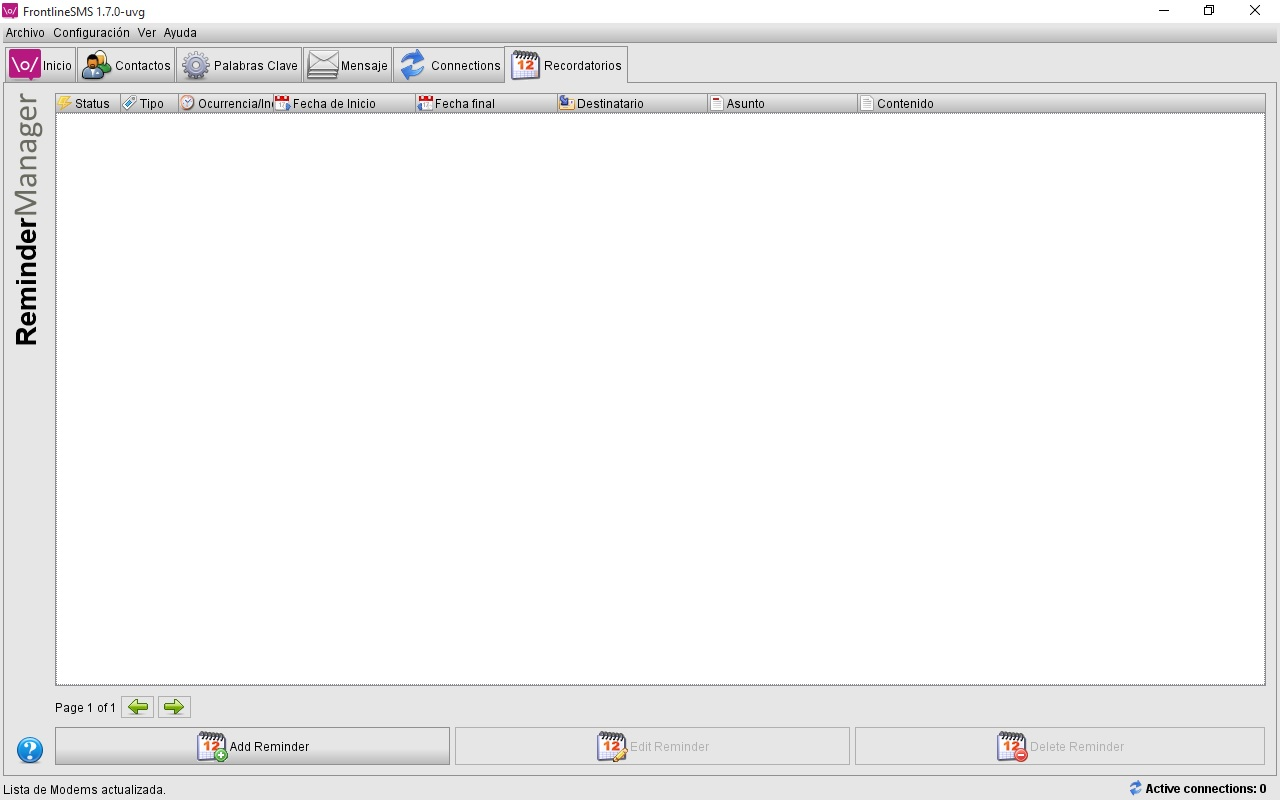
\includegraphics[height=7cm]{frontlinesms6.jpg}
         		\caption{Pantalla de recordatorios de FrontlineSMS}
         		\label{fig:frontline-sms2}
         	\end{center}
\end{figure}

En la Figura \ref{fig:frontline-sms2} se describe la pantalla de recordatorios que est�n en cola esperando a ser enviados y trasladados al buz�n de mensajes. Estos recordatorios tambi�n pueden ser filtrados por fecha, paciente y estatus.\\ \\ \\ \\


\subsubsection{Integraci�n de FrontlineSMS con OpenMRS} 

Como parte del dise�o del sistema de informaci�n al paciente, se contempl� la integraci�n de las plataformas FronlineSMS y OpenMRS. Para ello se propone el uso de una aplicaci�n de mensajer�a para que OpenMRS pueda compartir sus datos a FrontlineSMS. La soluci�n hace uso de servicios web Figura \ref{fig:frontline-openmrs-mensajeria}.\\

\begin{figure}[h]
         	\begin{center}
         		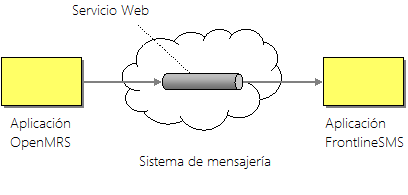
\includegraphics{message-solution.png}
         		\caption{Soluci�n de la comunicaci�n entre FrontlineSMS y OpenMRS}
         		\label{fig:frontline-openmrs-mensajeria}
         	\end{center}
\end{figure}

Para lograr integrar las dos plataformas, se segui� el patr�n de integraci�n adaptador. De esta forma se puede acceder a la base de datos de OpenMRS por medio de la creaci�n de la API que simplemente est� compuesta por servicios web. El dise�o resultante del sistema de informaci�n al paciente se presenta en la Figura \ref{fig:frontline-openmrs-adapter}. Todo comienza desde que la secretaria y el m�dico ingresan los datos a OpenMRS, luego los datos viajan por servicios web hasta llegar a la base de datos de FrontlineSMS. Por �ltimo, los recordatorios automatizados con informaci�n importante llegan a los pacientes. 

\begin{figure}[h]
         	\begin{center}
         		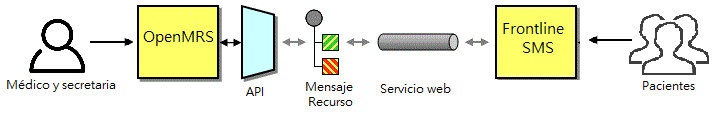
\includegraphics[width=11.5cm]{sistema-comunicacion.png}
         		\caption{Aplicaci�n del patr�n de integraci�n Adaptador entre FrontlineSMS y OpenMRS}
         		\label{fig:frontline-openmrs-adapter}
         	\end{center}
\end{figure}




%  % % % % % % % % % % % % % % % % % % % % % % % % % % % % % % % % % % % %
%
%                                                               Analisis de Resultados
% % % % % % % % % % % % % % % % % % % % % % % % % % % % % % % % % % % % %
%\setcounter{chapter}{15}% Equivalent to "letter O"
\renewcommand{\thechapter}{\Alph{chapter}}
\Chapter{An�lisis de resultados}


\justify
\section{Clasificaci�n de las carreras tentativas}

\begin{table}[H]
	\begin{center}
		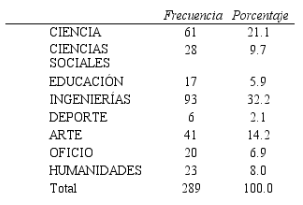
\includegraphics{clasificacionTentativas}
		\caption{Frecuencia y porcentaje de los estudiantes seg�n sus categor�as de carrera tentativa}
		\label{fig:clasificacionTentativas}
	\end{center}
\end{table}

	Se clasificaron las respuestas que los estudiantes ingresaron en la encuesta en 8 categor�as. De esta manera, se logra encontrar a qu� rama pertenecen las carreras tentativas que los estudiantes de la Universidad manifiestan como favoritas. Se logra observar que la categor�a que m�s sobresale es la ingenier�a y en segundo la categor�a ciencia. Muchos de estos ingenieros, si bien es cierto est�n cursando una carrera de esta �ndole, preferir�an estar en otro tipo de ingenier�a, pero muchos de ellos debido a factores externos se ven obligados a seguir otra ingenier�a. Por otra parte, algunos de ellos manifestaron estar a gusto con su carrera, sin embargo la carrera que cursan tiene relaci�n o servir� de conexi�n para llegar a la ingenier�a que realmente desean seguir. De igual manera, dicha respuesta aplica para ciencias puras, ya que algunos mencionan que su ingenier�a les sera de utilidad para cursar alguna carrera mas aplicada a lo cient�fico. Por �ltimo, las 3 facultades restantes est�n sus respuestas est�n dispersas en las categor�as restantes.\\


\section{Correlaci�n entre carreras tentativas y universitarias}

\begin{table}[H]
	\begin{center}
		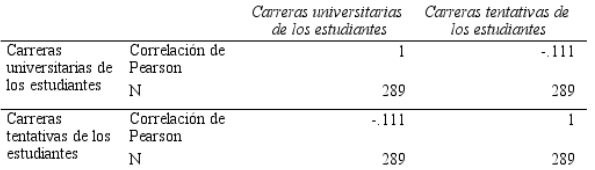
\includegraphics{correlacionTentativa}
		\caption{Correlaci�n entre la categor�a de las carreras tentativas y las universitarias de los estudiantes}
		\label{fig:correlacionTentativa}
	\end{center}
	\end{table}


\section{Estudiantes que encuentran una relaci�n entre carrera tentativa y universitaria}

\begin{figure}[H]
	\begin{center}
		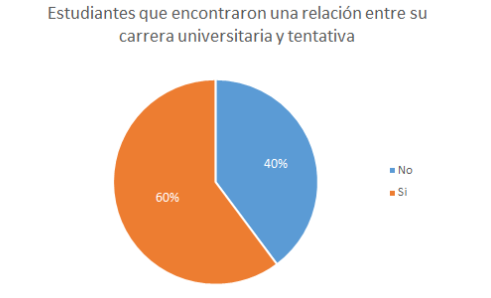
\includegraphics{encontraronRelacion}
		\caption{Estudiantes de la UVG que encontraron una relaci�n entre su carrera tentativa y universitaria}
		\label{fig:encontraronRelacion}
	\end{center}
\end{figure}


\section{Estudiantes que encuentran una relaci�n entre carrera tentativa y universitaria}

\begin{figure}[H]
	\begin{center}
		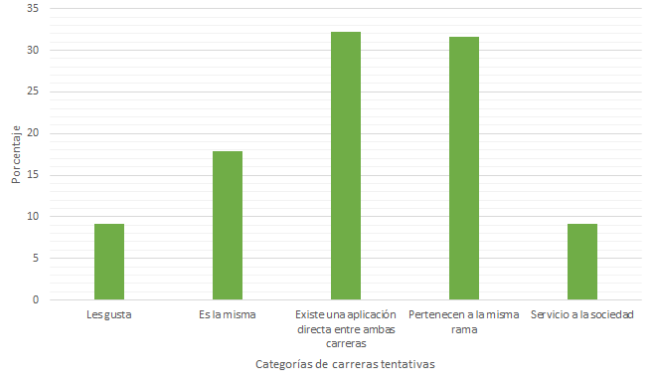
\includegraphics{categoriasRelaciones}
		\caption{Categorizaci�n de las relaciones entre la carrera tentativa y universitaria encontradas por los estudiantes}
		\label{fig:categoriasRelaciones}
	\end{center}
\end{figure}


\section{Satisfacci�n de los estudiantes con su carrera universitaria}

\begin{figure}[H]
	\begin{center}
		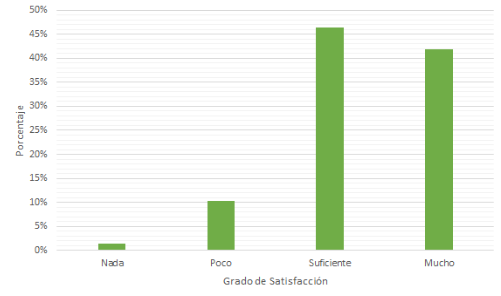
\includegraphics{gradoSatisfaccion}
		\caption{Grado de satisfacci�n de los estudiantes de la UVG con su carrera universitaria}
		\label{fig:gradoSatisfaccion}
	\end{center}
\end{figure}


\section{Estudiantes que escogieron su carrera tentativa como universitaria}

\begin{figure}[H]
	\begin{center}
		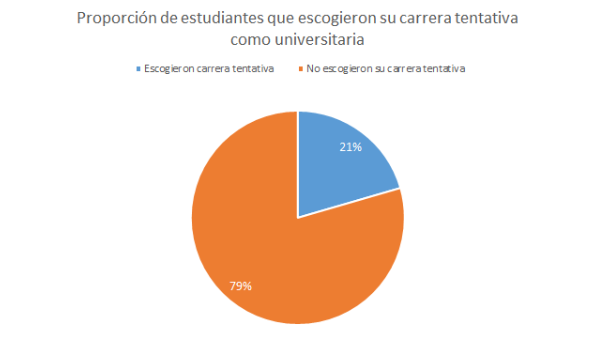
\includegraphics{tentativaUniversitaria}
		\caption{Proporci�n de los estudiantes que escogieron su carrera tentativa como universitaria}
		\label{fig:tentativaUniversitaria}
	\end{center}
\end{figure}

\begin{table}[H]
	\begin{center}
		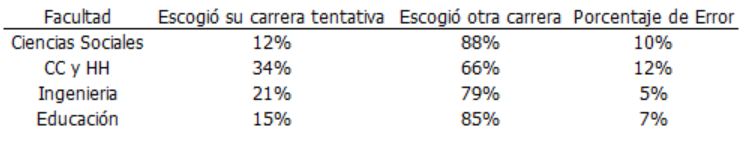
\includegraphics{tentativaUniversitariaFacultad}
		\caption{Porcentaje de estudiantes de la UVG que escogieron su carrera de etapa tentativa como universitaria seg�n su facultad}
		\label{fig:tentativaUniversitariaFacultad}
	\end{center}
\end{table}


\section{Influencia de ciertos factores en la elecci�n de carrera universitaria}

\begin{table}[H]
	\begin{center}
		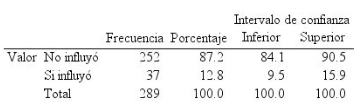
\includegraphics{factorPopularidad}
		\caption{Estudiantes que indicaron que el factor popularidad de la carrera los influenci�}
		\label{fig:factorPopularidad}
	\end{center}
\end{table}
Como se puede observar los estudiantes de la Universidad del Valle consideran que el factor popularidad es el que menos los influencia a la elecci�n de su carrera, por lo que se puede decir que es factor casi despreciable ya que la proporci�n de personas que considera que si influencio se estima que esta entre 9.5\% y 15.9\%.
\begin{table}[H]
	\begin{center}
		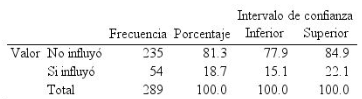
\includegraphics{factorPadres}
		\caption{Estudiantes que indicaron que el factor influencia de los padres o encargados los influenci�}
		\label{fig:factorPadres}
	\end{center}
\end{table}

En cuanto a los factor de padres o encargados, se obtuvo que es uno de los factores que menos influencia, ya que se estima que la proporci�n de estudiantes que lo considera se encuentra entre 15.1\% y 22.1\%. Por lo que se puede concluir que los padres o encargados no intervienen en su mayor�a en la elecci�n de carrera de los estudiantes.

\begin{table}[H]
	\begin{center}
		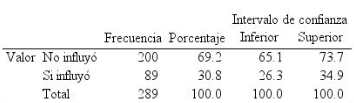
\includegraphics{factorRemuneracion}
		\caption{Estudiantes que indicaron que el factor remuneraci�n de la carrera los influenci�}
		\label{fig:factorRemuneracion}
	\end{center}
\end{table}

En cuanto al factor de remuneraci�n, aunque sea el segundo factor que m�s influencia a los estudiantes de la universidad, incre�blemente alrededor del 65.1\% y 73.7\% considera que es un factor que interviene en la elecci�n de carrera.

\begin{table}[H]
	\begin{center}
		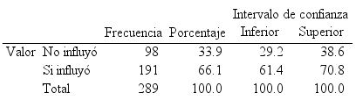
\includegraphics{factorOportunidad}
		\caption{Estudiantes que indicaron que el factor oportunidad laboral de la carrera los influenci�}
		\label{fig:factorOportunidad}
	\end{center}
\end{table}

Por �ltimo se encuentra el factor de oportunidad laboral, como se puede observar en el cuadro, es el factor el cual los estudiantes de la Universidad del Valle m�s consideran, ya que la proporci�n se encuentra entre el 61.4\% y 70.8\%, con esto se puede decir que el estudiante universitario al seguir su carrera considera que va a tener un trabajo asegurado al ser egresado de la universidad.

\section{Distribuci�n de carreras tentativas seg�n el sexo del estudiante}

\begin{table}[H]
	\begin{center}
		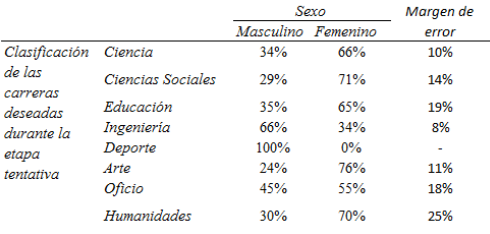
\includegraphics{SexoTentativa}
		\caption{Cuadro de contingencia entre sexo y categor�a de carrera tentativa del estudiante}
		\label{fig:SexoTentativa}
	\end{center}
\end{table}


\section{Correlaci�n entre influencia de los padres y posibilidad de elecci�n de carrera de los estudiantes}

\begin{table}[H]
	\begin{center}
		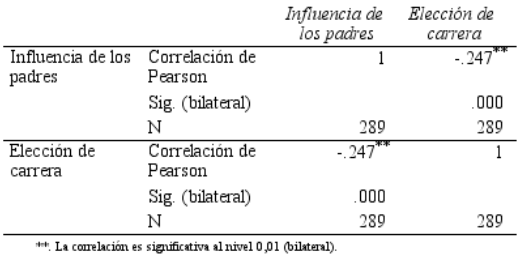
\includegraphics{padresEleccion}
		\caption{Correlaci�n entre el grado de influencia de los padres y si los estudiantes escogieron su carrera}
		\label{fig:padresEleccion}
	\end{center}
\end{table}

Como se puede observar en la figura, se tiene la correlaci�n para poder analizar la hip�tesis alternativa, seg�n los resultados se tiene una correlaci�n seg�n la escala de Pearson de -0.247, siendo esta una correlaci�n significativa, por lo que la hip�tesis alternativa se rechaza, ya que se obtuvo que entre m�s influencien los padres a sus hijos es menos probable que ellos elijan su carrera universitaria.




%  % % % % % % % % % % % % % % % % % % % % % % % % % % % % % % % % % % % %
%
%                                                              Conclusiones
% % % % % % % % % % % % % % % % % % % % % % % % % % % % % % % % % % % % %
%%  % % % % % % % % % % % % % % % % % % % % % % % % % % % % % % % % % % % %
%
%                                                              Conclusiones
% % % % % % % % % % % % % % % % % % % % % % % % % % % % % % % % % % % % %
\Chapter{Conclusiones}

\begin{itemize}

\item Es claro que existen ya millones de herramientas que han sido creadas para el �rea de salud, pero \emph{�cu�ntas de estas se adaptan al sector p�blico de Guatemala?}. La innovaci�n de este trabajo fue establecer el dise�o del sistema en base a las necesidades identificadas directamente en Guatemala. 

\item A partir de la investigaci�n realizada hasta la fase de exploraci�n, fue posible encontrar las cinco �reas de necesidad que presentaban los hospital en estudio.

\item Se gener� un prototipo refinado seg�n la metodolog�a de \emph{design thinking}, haciendo uso de la tecnolog�a necesaria para mejorar la atenci�n que reciben los pacientes en los hospitales p�blicos de Guatemala. Todo ello a partir del recorrido completo de la metodolog�a durante un per�odo de 10 meses.

\item Se dise�� un sistema de informaci�n, que establece una comunicaci�n que va desde el hospital hacia el paciente. Utilizando como canal de comunicaci�n entre ellos el servicio de mensajer�a corta el cual todos los tel�fonos m�viles poseen. 

\item Se dise�� un sistema de informaci�n, que establece una comunicaci�n que va desde el hospital hacia el paciente. Utilizando como canal de comunicaci�n entre ellos el servicio de mensajer�a corta el cual todos los tel�fonos m�viles poseen. 

\item El presente trabajo no s�lo propone al �rea de salud p�blica de Guatemala tecnolog�as de bajos recursos, sino que provee a la comunidad de desarrolladores el dise�o de un prototipo que integra las plataformas OpenMRS y FrontlineSMS.
\end{itemize}

%  % % % % % % % % % % % % % % % % % % % % % % % % % % % % % % % % % % % %
%
%                                                               Recomendaciones
% % % % % % % % % % % % % % % % % % % % % % % % % % % % % % % % % % % % %
%%  % % % % % % % % % % % % % % % % % % % % % % % % % % % % % % % % % % % %
%
%                                                               Recomendaciones
% % % % % % % % % % % % % % % % % % % % % % % % % % % % % % % % % % % % %

\Chapter{Recomendaciones}
Se deja como recomendaci�n los siguientes puntos:\\

\begin{itemize}
\item Tomar un curso sobre �tica y los pasos que se deben de seguir al realizar investigaci�n que involucra a sujetos humanos. y para futuras generaciones se debe considerar siempre someter todos los protocolos de trabajo de graduaci�n a un comit� de �tica desde el inicio del trabajo. \\

\item Realizar un plan desde el inicio de la investigaci�n para la comunicaci�n con los hospitales a estudiar. Esto se qued� como lecci�n por parte del grupo ya que la investigaci�n se vio retrasada en un punto por la gesti�n de todos los permisos de entrada y validaci�n de datos.
\item Completar la implementaci�n de todos los m�dulos generados. Debido a la informaci�n recopilada en los tres hospitales p�blicos, donde se realiz� este trabajo, fue posible observar que la necesidad de tecnolog�a en esta �rea es grande. Por lo tanto, se exhorta a la continuaci�n de este proyecto para cualquier hospital p�blico o privado.\\

\item Entrevistar equitativamente a todos los perfiles que se definen en la metodolog�a de \emph{design thinking}. De esta forma es posible evitar cualquier sesgo en la cantidad de necesidades que surgen durante las entrevistas. \\

\end{itemize}


%  % % % % % % % % % % % % % % % % % % % % % % % % % % % % % % % % % % % %
%
%                                                               Bibliografia
% % % % % % % % % % % % % % % % % % % % % % % % % % % % % % % % % % % % %

\Biblio
\begin{thebibliography}{9}
\Bibliotoc


\bibitem[Acevedo \& Alvarado (2008)]{Acevedo2008} Acevedo, M. \& Alvarado, C. (2008). \textit{Lecciones de Semiolog�a}, Sexta Edici�n. Guatemala.

\bibitem[Ambrose \& Harris (2010)]{dt-ambrose}
Ambrose, G. \& Harris, P. 2010. \textit{Design Th!nking}. Ava Publishing.

\bibitem[Becerril-Montekio \& L�pez-D�vila (2011)]{becerril-lopez} Becerril-Montekio, V�ctor y L. L�pez-D�vila. 2011. �Sistema de Salud en Guatemala� \textit{Salud P�blica Mex} \underline{LIII} (2): S197-S208.

\bibitem[California Research Bureau (2012)]{open-source-2}
California Research Bureau. 2012. \textit{Open-Source Software: Value, Cost, and Supporting Open Government} Recuperado de \url{https://www.library.ca.gov/crb/12/S-12-02.pdf}

\bibitem[Carnicero \& Fern�ndez (2011)]{dt-carnfern} Carnicero, J. \& Fern�ndez, A. 2011. \textit{Manual de salud electr�nica para directivos de servicios y sistemas de salud}. Santiago de Chile, Naciones Unidas. 414 p\'ags.

\bibitem[Castro \& G�mez (2002)]{Castro2002}Castro, L. \& G�mez, M. (2002). \textit{Historia cl�nica}. In Farmacia Hospitalaria - Tomo I (pp. 295 - 305). Espa�a: Sociedad Espa�ola de Farmacia Hospitalaria. Recuperado de \url{http://www.sefh.es/bibliotecavirtual/fhtomo1/cap22.pdf}

\bibitem[Coiera (2006)]{Coiera2006}Coiera, E. (2006). \textit{Communication systems in healthcare}. The Clinical Biochemist. Reviews / Australian Association of Clinical Biochemists, 27(2), 89?98.

\bibitem[Blakely \& Timmons (2008)]{bla-timm}
Blakely, M., \& Timmons, S. 2008. \textit{Life Style and Health Research}. New York: Nova.

\bibitem[Cottom (2004)]{cottom}Cottom, Hugo. 2004. \textit{An�lisis cr�tico del sistema nacional de salud en Guatemala}. Tesis Universidad Rafael Land�var. Quetzaltenango, Guatemala. 12 p�gs.

\bibitem[Dhanshetti (2015)]{dhanshetti}
Dhanshetti, S. 2015. \textit{Communication system}. Maharashtra: Industrial Training Institute.

\bibitem[Dunlop et al. (2013)]{dunlop}
Dunlop, J., Girma, D., \& Irvine, J. 2013. \textit{Digital Mobile Communications and the TETRA System}. West Sussex: John Wiley \& Sons.

\bibitem [Dutoit (1997)]{dutoit}
Dutoit, T. 1997. \textit{An Introduction to Text-to-Speech Synthesis}. (Vol. 3). Dordrecht: Springer Netherlands. http://doi.org/10.1007/978-94-011-5730-8

\bibitem [de la Harpe, Kabaso, \& Debrah (2014)]{harpe-ko}
De la Harpe, R., Kabaso, B., \& Debrah, R. 2014. \textit{Design of mobile appointment reminder and counselling system}. In Proceedings of the 9th Health Informatics in Africa Conference HELINA'14 (pp. 39-45). Koegni eHealth. Retrieved from \url{http://helina-online.org/}

\bibitem [Downer, Meara, Da Costa, \& Sethuraman (2006)]{downer-mea}
Downer, S., Meara, J., Da Costa, A., \& Sethuraman, K. 2006. \textit{SMS text messaging improves outpatient attendance}. Australian Health Review: A Publication of the Australian Hospital Association, 30(3), 389-396. \url{http://doi.org/10.1071/AH060389}

\bibitem [Egan (1993)]{egan-t}
Egan, T. 1993. \textit{Using Interactive Voice Response Systems. In Beyond Computing and Connectivity}. West Chester: DIANE Publishing Company. Pp. 391-399.

\bibitem [Emol (2015)]{bench-apple}
Emol. 2015. \textit{Apple expande tecnolog�a para la salud en principales hospitales de Estados Unidos}. Recuperado de \url{http://www.emol.com/noticias/tecnologia/2015/02/05/702418/apple-expande-tecnologia-de-salud-en-principales-hospitales-de-estados-unidos.html}

\bibitem [Frehner (2008)]{frehner-c}
Frehner, C. 2008. \textit{Email, SMS, MMS: The Linguistic Creativity of Asynchronous Discourse in the New Media Age}. Bern: Peter Lang.

\bibitem [FrontlineSMS (2009)]{front-2009}
FrontlineSMS. 2009. \textit{Celebrating the art of the possible}. Retrieved October 1, 2015, from \url{http://www.frontlinesms.com/2009/11/19/celebrating-the-art-of-the-possible/}

\bibitem [FrontlineSMS (2011)]{front-2011}
FrontlineSMS. 2011. \textit{User Guide: Data Integrity}, 1?65. Obtenido de \url{http://www.frontlinesms.com/wp-content/uploads/2011/08/frontlinesms_userguide.pdf}

\bibitem [FrontlineSMS (2015)]{front-2015}
FrontlineSMS. 2015. \textit{FrontlineSMS Overview}. Recuperado el August 1, 2015, from \url{http://www.frontlinesms.com/technologies/frontlinesms-overview/}

\bibitem [Grover, Stewart, Lubensky, Hare, \& Jai (2012)]{grover-stewart}
Grover, A. S., Stewart, O., Lubensky, D., Hare, K., \& Jai, P. 2009. \textit{Designing Interactive Voice Response (IVR) Interfaces: localisation for low literacy users}. In Proceedings of Computers and Advanced Technology in Education (p. 8). St Thomas.

\bibitem [Gestwicki y McNely (2012)]{dt-gestwicki}
Gestwick, P. \& Mcely, B.  2013. \textit{A case study of a five-step design thinking process in educational museum game design}. Recuperado de \url{http://meaningfulplay.msu.edu/proceedings2012/mp2012_submission_37.pdf}

\bibitem [Haji, Suleman, \& Rivett (2015)]{haji-su}
Haji, H., Suleman, H., \& Rivett, U. 2015. \textit{Development of a Mobile Image-Based Reminder Application to Support Tuberculosis Treatment in Africa}. International Journal of Medical, Health, Biomedical, Bioengineering and Pharmaceutical Engineering, 9(8), 522-529.

\bibitem [Herrera (2012)]{herrera-w}
Herrera, J. 2012. \textit{Nuevas tendencias en comunicaci�n}. 2da ed. Madrid: ESIC.

\bibitem [Hospital Roosevelt (2015)]{ho-roo}
Hospital Roosevelt. 2015. \textit{Hospital Roosevelt Gobierno de Guatemala}. Recuperado el 16 de septiembre de 2015, de \url{http://www.hospitalroosevelt.gob.gt/hr/}

\bibitem [Hospital San Juan de Dios (2015)]{ho-sanjuan}
Hospital San Juan de Dios. 2015. \textit{Hospital General San Juan de Dios}. Recuperado el 16 de septiembre de 2015, de \url{http://www.hospitalsanjuandediosguatemala.com/pages/inicio.php#.Vfnh0_l_Oko} 

\bibitem[IDEO's Attributions (2012)]{dt-ideos}
IDEO's Attributions. 2012. \textit{Design Thinking for Educators}, segunda ed. IDEO.

\bibitem [ISSSTE (2005)]{bench-issste}
ISSSTE. 2005. \textit{Sistema de cita m�dica telef�nica e internet}. Recuperado de \url{http://189.254.143.89/issste/comun/home.aspx}

\bibitem [Huckvale, Prieto, Tilney, Benghozi, \& Car (2015)]{jose-tomas}
Huckvale, K., Prieto, J. T., Tilney, M., Benghozi, P.-J., \& Car, J. 2015. \textit{Unaddressed privacy risks in accredited health and wellness apps: a cross-sectional systematic assessment}. BMC Medicine, 13(1), 214. \url{http://doi.org/10.1186/s12916-015-0444-y}

\bibitem [Kuo, Lee, \& Tian (2006)]{kuo-lee}
Kuo, S., Lee, B., \& Tian, W. 2006. \textit{Real-Time Digital Signal Processing: Implementations and Applications}. 2nd ed., West Sussex: John Wiley \& Sons. 

\bibitem[Management Study Guide (2013)]{ManagementStudyGuide2013}
Management Study Guide. 2013. \textit{Components of Communication Process}. De \url{http://www.managementstudyguide.com/components-of-communication-process.htm}

\bibitem [Martinez-Fernandez et al. (2015)]{marti-fer} 
Martinez-Fernandez, A., Lobos-Medina, I., Diaz-Molina, C., Chen-Cruz, M., \& Prieto-Egido, I. 2015. \textit{TulaSalud: An m-health system for maternal and infant mortality reduction in Guatemala}. Journal of Telemedicine and Telecare, 21(5), 283-291. \url{http://doi.org/10.1177/1357633X15575830}

\bibitem [McDonald (2014)]{mc-donald}
McDonald, L. W. 2014. \textit{Sexual Exploitation Outreach with Text Messaging: Introducing Project Backpage}. Retrieved September 6, 2015, from \url{http://www.frontlinesms.com/2014/01/29/sexual-exploitation-outreach-with-text-messaging-introducing-project-backpage/}


\bibitem [Ministerio de Salud P�blica y Asistencia Social (2013)]{hospital}
Ministerio de Salud P�blica y Asistencia Social. 2013. \textit{Auditor�a Financiera: Hospital Infantil de Infectolog�a y Rehabilitaci�n}. Recuperado el 07 de julio de 2015, de \url{http://www.mspas.gob.gt/libreacceso/images/stories/datos/2013/ABRIL%20UIP%202013/Art.%2010%20numeral%2023.%20Auditor%C3%ADas%20realizadas/CUA-22622%20(Hospital%20Infantil%20e%20Infectolog%C3%ADa).pdf}

\bibitem [Moller \& Bort (1993)]{moeller-bort}
Moeller, M. \& Bort, J. 1993. \textit{VM gets the message. Communications International}, 20, 14-15. 

\bibitem[Nist (2014)]{Nist2014}
Nist. (2014). \textit{Framework for Improving Critical Infrastructure Cybersecurity}, 39. Recuperado de \url{http://www.nist.gov/cyberframework/upload/cybersecurity-framework-021214.pdf}

\bibitem [Noar \& Harrington (2012)]{noar-harring}
Noar, S., \& Harrington, N. 2012. \textit{eHealth Applications Promising Strategies for Behavior Change}. New York: Routledge. 

\bibitem [OpenMRS (2015)]{opem-mrs-2015}
OpenMRS. 2015. \textit{Frequently Asked Questions}. Retrieved October 10, 2015, from \url{http://openmrs.org/about/faq/} 

\bibitem [Piette. et al. (2013)]{piette-mar}
Piette, J., Marinec, N., Gallegos-Cabriales, E., Gutierrez-Valverde, J., Rodriguez-Saldana, J., Mendoz-Alevares, M., \&  Silveira, M. 2013. \textit{Spanish-speaking patient?s engagement in interactive voice response (IVR) support calls for chronic disease self-management: data from three countries}. Journal of Telemedicine and Telecare, 19(2), 89-94. \url{http://doi.org/10.1177/1357633X13476234}

\bibitem [Pitkin (2014)]{pit-a}
Pitkin, A. 2014. \textit{Technology Volunteerism for Social Good; How we made Frontline easier to use}. Retrieved September 5, 2015, from \url{http://www.frontlinesms.com/2014/12/23/sc4g-multiselector/}

\bibitem [Razzouk y Shute (2012)]{dt-razzouk}
Razzouk, R. \& Shute, V.  2013. \textit{What Is Design Thinking and Why Is It Important?}. Recuperado de \url{http://myweb.fsu.edu/vshute/pdf/designthinking.pdf}

\bibitem [Salus (2013)]{bench-salus}
Salus. 2013. \textit{Salus: Software para hospitales y cl�nicas}. Recuperado de \url{http://www.softwaresalus.com/DefaultSalus.aspx}

\bibitem[Santizo (2010)]{santizo-firma}
Santizo, J. 2010. \textit{Implementaci�n y adopci�n de la firma electr�nica en Guatemala}. Universidad de San Carlos de Guatemala.

\bibitem[Scholl et al (2008)]{Scholl2008}
Scholl, M. a, Stine, K. M., Hash, J., Bowen, P., Johnson, L. A., Smith, C. D., \& Steinberg, D. I. (2008). \textit{An Introductory Resource Guide for Implementing the Health Insurance Portability and Accountability Act (HIPAA) Security Rule}, (October). Recuperado de \url{http://csrc.nist.gov/publications/nistpubs/800-66-Rev1/SP-800-66-Revision1.pdf}

\bibitem[Stair \& Reynolds (2015)]{stair-rey}
Stair, R., \& Reynolds, G. 2015. \textit{Principles of Information Systems}. 12va ed. Boston: Cengage Learning.

\bibitem [Jo Woc (2005)]{jo-woc}
Stephen Jo Woc. 2005. \textit{Ampliaci�n Y Remodelaci�n de la Consulta Externa de Adultos Del Hospital Roosevelt}. Universidad de San Carlos de Guatemala. Recuperado el 16 de septiembre de 2015, de \url{http://biblioteca.usac.edu.gt/tesis/02/02_1337.pdf} 

\bibitem [Stickel (2013)]{stick-c}
Stickel, C. 2013. \textit{FrontlineSMS Named 1 Tech NGO in the World by the Global Journal}. Retrieved September 1, 2015, from \url{http://www.frontlinesms.com/2013/07/24/frontlinesms-named-1-tech-ngo-in-the-world-by-the-global-journal/}

\bibitem [Swiss Tropical Institute (2015)]{swiss-trop}
Swiss Tropical Institute. 2015. eHealth Toolbox. Retrieved September 15, 2015, from http://www.swisstph.ch/services/ehealth/ehealth-toolbox.html

\bibitem [TechTimes (2015)]{bench-kit}
TechTimes. 2015. \textit{Apple HealthKit App launching in top US hospitals}. Recuperado de \url{http://www.techtimes.com/articles/31049/20150205/apple-healthkit-app-launching-in-top-us-hospitals.htm}

\bibitem [Trisby, Holley, \& Harris (2010)]{tris-h}
Trisby, F., Holley, K., \& Harris, I. 2010. \textit{Short Message Service(SMS) the creation of personal global text messaging}. Vasa. West Sussex: John Wiley \& Sons. Recuperado de \url{http://medcontent.metapress.com/index/A65RM03P4874243N.pdf}

\bibitem [Universidad de San Carlos de Guatemala (2014)]{bench-balanza}
Universidad de San Carlos de Guatemala. 2014. \textit{Evaluaci�n de un medidor electr�nico antropom�trico b�sico para ni�os mayores a 6 a�os que automatice la lectura y registro de datos}. Recuperado de \url{http://digi.usac.edu.gt/bvirtual/informes/puicb/INF-2013-21.pdf}

\bibitem[Verizon (2015)]{Verizon2015}
Verizon. (2015). \textit{2015 Data Breach Investigations Report}. Information Security, 1-70. Recuperado de \url{http://www.verizonenterprise.com/DBIR/2015/}

\bibitem [Virji et al. (2006)]{virji-bbc}
Virji, A., Yarnall, K., Krause, K., Pollak, K., Scannell, M., Gradison, M., \& Ostbye, T. 2006. \textit{Use of email in a family practice setting: opportunities and challenges in patient- and physician-initiated communication}. BMC Medicine, 4(1), 18. \url{http://doi.org/10.1186/1741-7015-4-18}

\bibitem [Visionstate (2013)]{bench-wanda}
Visionstate. 2013. \textit{WANDA restroom management}. Recuperado de \url{http://visionstate.com/wanda/}

\bibitem [Weerawarana y Weeratunga (2004)]{opensource}
Weerawarana, S., \& Weeratunga, J. 2004. \textit{Open Source in Developing Countries}. Recuperado de \url{http://www.eldis.org/fulltext/opensource.pdf}

\bibitem [Weldon et al.(2014)]{weldon-fran}
Weldon, C., Francois, T., Trosman, J., Roggenkamp, B., Dupuy, D., Knight, J., ? Murphy, A. 2014. \textit{Abstract A84: Do patient follow-up improvements, at hospitals caring for medically underserved patients, impact no-show rates}. Cancer Epidemiology Biomarkers \& Prevention, 23(11 Supplement), A84-A84. \url{http://doi.org/10.1158/1538-7755.DISP13-A84}

\bibitem [Witten \& Madams (1977)]{witten-madams}
Witten, I. H., \& Madams, P. H. C. 1977. \textit{The telephone enquiry service: a man-machine system using synthetic speech}. International Journal of Man-Machine Studies, 9, 449-64.

\bibitem [Witter, Steele, Mcewen, \& Mehler (2001)]{witter-st}
Witter, J., Steele, A., Mcewen, D., \& Mehler, P. 2001. \textit{The Effect of Computer Generated Appointment Reminders On Compliance With Clinic Appointments}. The Internet Journal of Healthcare Administration, 8(2), 1-5. Retrieved from \url{http://ispub.com/IJHCA/8/2/10328#}

\bibitem [Wolfe \& Korytkowsk (2013)]{wolfe-kory13}
Wolfe, B., \& Korytkowsk, R. 2013.  \textit{REST Web Services Technical Documentation}. Retrieved October 4, 2015, from \url{https://wiki.openmrs.org/display/docs/REST+Web+Services+Technical+Documentation}

\bibitem [Wolfe \& Korytkowsk (2015)]{wolfe-kory}
Wolfe, B., \& Korytkowsk, R. 2015. \textit{REST Module}. Retrieved October 4, 2015, from \url{https://wiki.openmrs.org/display/docs/REST+Module}

\bibitem [Wolfe \& Purkayastha (2015)]{wolfe-purka}
Wolfe, B., \& Purkayastha, S. 2015. \textit{REST Web Services API For Clients}. Retrieved October 4, 2015, from \url{https://wiki.openmrs.org/display/docs/REST+Web+Services+API+For+Clients}

\bibitem [Yarberry (2002)]{yarberry-w}
Yarberry, W. 2002. \textit{Interactive Voice Response. In Computer Telephony Integration}. 2nd ed., pp. 79-89. Boca Rat�n: CRC Press.

\bibitem [Yetisen et al. (2014)]{yetisen-m}
Yetisen, A. K., Martinez-Hurtado, J. L., da Cruz Vasconcellos, F., Simsekler, M. C. E., Akram, M. S., \& Lowe, C. R. 2014.  \textit{The regulation of mobile medical applications}. Lab on a Chip, 14(5), 833. \url{http://doi.org/10.1039/c3lc51235e}

\bibitem [6inf (2013)]{bench-his}
6inf. 2013. \textit{TESIS HIS}. Recuperado el 07 de julio de 2015, de \url{http://www.sisinf.com/es/his-software-para-hospitales.php}


\bibitem [Instituto Nacional de Estad�stica (2012)]{ine}
21. Instituto Nacional de Estad�stica. 2012. \textit{Proyecciones de INE al 30 de julio del 2012.} Recuperado de \url{http://www.ine.gob.gt/sistema/uploads/2014/02/26/5eTCcFlHErnaNVeUmm3iabXHaKgXtw0C.pdf}

\bibitem [Stead y Lin (2009)]{prefacio-2} Stead, W. y H. Lin. 2009. \textit{Computational technology for effective health care: immediate steps and strategic directions}. The National Academies Press. Recuperado de \url{https://www.nlm.nih.gov/pubs/reports/comptech_2009.pdf}

\bibitem [Fett (2000)]{techonolog-care}
Fett, M. 2000. \textit{International Technology , approaches to funding health care Care Health and Health}. Health Financing Series, 5, 42.

\bibitem [Stead \& Lin (2009)]{fett-lin}
Stead, W., \& Lin, H. S. 2009. \textit{Computational technology for effective health care immediate steps and Strategic directions}.

\end{thebibliography}


%  % % % % % % % % % % % % % % % % % % % % % % % % % % % % % % % % % % % %
%
%                                                               Anexos
% % % % % % % % % % % % % % % % % % % % % % % % % % % % % % % % % % % % %
\Chapter{Anexos}

\section{Entrevistas semi-estructuradas basadas en el brief del estudio}
dfdfdfd\\

\end{document}

